% !TeX program = xelatex
% Optional supplementary document. main.tex is the manuscript.
\RequirePackage[T1]{fontenc}
\RequirePackage{xcolor}
\documentclass[journal,twoside,web]{ieeecolor}
\usepackage{xcolor}\usepackage{jsen}
% No geometry/titlesec/fancyhdr overrides: layout is owned by ieeecolor + jsen.
\usepackage{iftex}
\ifPDFTeX
  % Compatibility path: pdfLaTeX must never load fontspec.
  \usepackage[T1]{fontenc}
  \usepackage{kotex}
  \DeclareUnicodeCharacter{2212}{\ensuremath{-}}
  \DeclareUnicodeCharacter{2192}{\ensuremath{\rightarrow}}
  \DeclareUnicodeCharacter{2194}{\ensuremath{\leftrightarrow}}
  \DeclareUnicodeCharacter{2264}{\ensuremath{\leq}}
  \DeclareUnicodeCharacter{2265}{\ensuremath{\geq}}
  \DeclareUnicodeCharacter{00D7}{\ensuremath{\times}}
\else
  \usepackage{fontspec}
  \usepackage{kotex}
  \IfFontExistsTF{TeX Gyre Termes}{\setmainfont{TeX Gyre Termes}}{\setmainfont{Liberation Serif}}
  \IfFontExistsTF{TeX Gyre Heros}{\setsansfont{TeX Gyre Heros}[SmallCapsFont={TeX Gyre Heros}]}{\setsansfont{Liberation Sans}[SmallCapsFont={Liberation Sans}]}
  \IfFontExistsTF{TeX Gyre Cursor}{\setmonofont{TeX Gyre Cursor}[Scale=MatchLowercase]}{\setmonofont{DejaVu Sans Mono}[Scale=MatchLowercase]}
  \IfFontExistsTF{UnBatang}{%
    \setmainhangulfont{UnBatang}[AutoFakeSlant=.15,SmallCapsFont=UnBatang]
  }{\setmainhangulfont{Noto Serif CJK KR}[AutoFakeSlant=.15,SmallCapsFont={Noto Serif CJK KR}]}
  \IfFontExistsTF{UnDotum}{%
    \setsanshangulfont{UnDotum}[AutoFakeSlant=.15,SmallCapsFont=UnDotum]
  }{\setsanshangulfont{Noto Sans CJK KR}[AutoFakeSlant=.15,SmallCapsFont={Noto Sans CJK KR}]}
  \IfFontExistsTF{UnDotum}{\setmonohangulfont{UnDotum}}{}
\fi
\usepackage{cite}
\usepackage{amsmath,amssymb,amsfonts,bm}
\usepackage{graphicx,booktabs,array,tabularx,multirow}
\usepackage{xcolor,wrapfig}
\usepackage{tikz}
\usetikzlibrary{arrows.meta,positioning,calc,fit,backgrounds}
\usepackage{url}
\usepackage{placeins,needspace}
\usepackage{etoolbox}
\usepackage[unicode,hidelinks]{hyperref}

% The unmodified class explicitly asks for LOGO-jsen-web.eps four times.
% Replace only that asset extension in memory; preserve all class geometry.
\makeatletter
\newcommand{\sensorslogopatch}{%
  \patchcmd{\ps@titlepagestyle}{\logoname.eps}{\logoname.pdf}{}%
    {\PackageError{sensors-compat}{Logo patch failed}{Use the supplied ieeecolor.cls.}}}
\sensorslogopatch\sensorslogopatch\sensorslogopatch\sensorslogopatch

% Korean-only compatibility: the legacy class hard-codes T1/Helvetica in
% section/table/figure headings. Keep its sizes/spacing/colors unchanged,
% but let Unicode engines select the configured Latin/Hangul sans families.
\ifPDFTeX\else
  \patchcmd{\section}{\fontencoding{T1}}{\normalfont\sffamily}{}{}
  \patchcmd{\section}{\fontfamily{phv}}{}{}{}
  \let\@IEEEappendixsavesection\section
  \patchcmd{\@makecaption}{\fontencoding{T1}}{\normalfont\sffamily}{}{}
  \patchcmd{\@makecaption}{\fontfamily{phv}}{}{}{}
  \patchcmd{\tablefont}{\fontencoding{T1}}{\normalfont\sffamily}{}{}
  \patchcmd{\tablefont}{\fontfamily{phv}}{}{}{}
  \patchcmd{\figfont}{\fontencoding{T1}}{\normalfont\sffamily}{}{}
  \patchcmd{\figfont}{\fontfamily{phv}}{}{}{}
\fi


\patchcmd{\@maketitle}{\sublargesize\sf\@author\centerline}{\sublargesize\sf\@author\par\centerline}{}{}
% Correct an author-line break and empty-caption tests in the supplied legacy
% class, without changing sizes, margins, column widths, or caption positions.
\patchcmd{\@makecaption}{\if #2}{\if\relax\detokenize{#2}\relax}{}{}
\patchcmd{\@makecaption}{\if #2}{\if\relax\detokenize{#2}\relax}{}{}
\patchcmd{\@makecaption}{\if #2}{\if\relax\detokenize{#2}\relax}{}{}
\patchcmd{\@makecaption}{\if #2}{\if\relax\detokenize{#2}\relax}{}{}

% Use LaTeX's color-aware savebox wrapper in figure captions.
% The legacy raw hbox loses color-stack scope when it is unboxed.
\patchcmd{\@makecaption}{\setbox\@tempboxa\hbox}{\sbox\@tempboxa}{}{}
\patchcmd{\@makecaption}{\setbox\@tempboxa\hbox}{\sbox\@tempboxa}{}{}
\makeatother

\definecolor{abstractbg}{rgb}{0.89804,0.94510,0.83137}
\definecolor{PendingBG}{HTML}{F2F3F5}
\definecolor{Muted}{HTML}{4D5962}
\setlength{\fboxrule}{0pt}
\setlength{\fboxsep}{0pt}
\setlength{\emergencystretch}{2em}
\newcolumntype{Y}{>{\raggedright\arraybackslash}X}
\newcommand{\pending}[1]{\par\smallskip\noindent\colorbox{PendingBG}{\parbox{\dimexpr\columnwidth-2\fboxsep\relax}{\small\textbf{[추정·미검증: 추가 검증]} #1}}\par\smallskip}
\newcommand{\draftnote}[1]{\par\smallskip\noindent{\small\color{Muted}\textbf{[확인 범위]} #1}\par\smallskip}
\newcommand{\R}{\mathbf R}
\newcommand{\tvec}{\mathbf t}
\newcommand{\pvec}{\mathbf p}
\newcommand{\uvec}{\mathbf u}
\newcommand{\K}{\mathbf K}
\newcommand{\dvec}{\mathbf d}
\newcommand{\vvec}{\mathbf v}
\newcommand{\notrun}{\textnormal{\sffamily x}}
\newcommand{\NA}{\textnormal{해당 없음}}
\newcommand{\tabnote}[1]{\par\vspace{3pt}\begin{minipage}{\linewidth}\footnotesize #1\end{minipage}}
\newcommand{\figpending}[2]{\fcolorbox{Muted}{PendingBG}{\parbox[c][#1][c]{\dimexpr\linewidth-2\fboxsep-2\fboxrule\relax}{\centering{\sffamily\Large x}\par\medskip{\footnotesize #2}}}}
\hypersetup{pdftitle={영상 특징과 치수 정보를 활용한 단안 팔레트 자세 추정용 국소 키포인트 보정},pdfauthor={Author information pending},pdfsubject={Korean manuscript revision 2026-10-06; original N3 snapshot preserved; independent metrology incomplete}}

% Vector assets use PDF 1.7; no raster conversion or shell-escape is needed.


\newcommand{\pckten}{\ensuremath{\mathrm{PCK}@10\mathrm{px}}}
\newcommand{\base}{\textnormal{Base}}

\hypersetup{pdftitle={팔레트 국소 키포인트 보정: 보충자료}}
\begin{document}
\renewcommand{\thetable}{S\Roman{table}}
\renewcommand{\thefigure}{S\arabic{figure}}
\title{영상 특징과 치수 정보를 활용한\\단안 팔레트 자세 추정용 국소 키포인트 보정\\보충자료}
\author{\mbox{저자 정보 확정 전}}
\markboth{\journalname, SUPPLEMENTARY MATERIAL}{PALLET KEYPOINT REFINEMENT: SUPPLEMENT}
\IEEEtitleabstractindextext{%
\fcolorbox{abstractbg}{abstractbg}{\begin{minipage}{\textwidth}
\begin{abstract}
본문의 중복을 줄이기 위해 이동한 상세 설정과 결과를 제시한다. 자료·평가 규칙·원수치는 본문과 같으며, 본문의 고정 자료를 사용하며, 별도 12장 PnP 보조 기하 참조의 탐색 패널은 공식 가시 코너 평가와 분리해 제시한다. 기본 추정기는 RGB만 받고 치수는 보정기와 자세 계산에서 사용한다. Base는 보정 없음, P는 별도 영상 보정 가중치, N0--N3는 통제 구성이다. 미확인 코너 가시성과 정사각형 가림 등급을 직접 가시 또는 clean으로 대체하지 않는다.
\end{abstract}
\begin{IEEEkeywords}보충 결과, 실험 설정, 팔레트 키포인트 보정.\end{IEEEkeywords}
\end{minipage}}}
\maketitle
\section{기반 추정기와 추가 보정 설정}
표~\ref{sup:backbone_contract}는 기반별 특징 채널·간격과 학습 대상을 정리한다. 모든 N3가 같은 물리적 치수 특징과 회전 대응 감독을 사용하지만 내부 특징 연결층과 보정 가중치는 별도로 학습한다. ResNet은 치수 문맥을 영벡터로 고정해 10 epoch 학습한 CONSTANT의 고정 특징 변환을 마지막 합성곱에 합친 RGB 모델이다. 별도 실제 치수 입력 FULL 모델을 본문의 Base로 사용하지 않았다.
\begin{table*}[t]
\centering\footnotesize
\caption{세 기반 추정기에 적용한 동일 N3 계약과 실행 상태. 초기 추정기와 치수를 받는 보정기를 구분한다.}
\label{sup:backbone_contract}
\setlength{\tabcolsep}{4pt}
\begin{tabularx}{\textwidth}{p{0.18\textwidth}YYY}
\toprule
항목 & YOLO26n & DOPE / VGG & ResNet-18 10-epoch RGB 변형 \\
\midrule
기본 신경망 입력 & RGB만 & RGB만 & RGB만 \\
연결부 특징 채널 / 간격 & (64,128) / (8,16) & (256,128) / (4,8) & (128,256) / (8,16) \\
N3 시각 정보 & 해당 특징·초기 코너·박스 & 해당 특징·초기 코너·박스 & 해당 특징·초기 코너·박스 \\
N3 물리적 치수 & 가로·깊이·높이 사용 & 가로·깊이·높이 사용 & 가로·깊이·높이 사용 \\
N3 학습 감독 & 전체 순열 선택 + 분포 손실 & 전체 순열 선택 + 분포 손실 & 전체 순열 선택 + 분포 손실 \\
보정 전후 PnP 정보 & 동일 카메라·치수 & 동일 카메라·치수 & 동일 카메라·치수 \\
학습하는 대상 & 연결부의 학습층·N3 헤드 & 기반별 연결 학습층·N3 헤드 & 기반별 연결 학습층·N3 헤드 \\
N3 학습·평가 완료 & 3 seed & 3 seed & 3 seed \\
\bottomrule
\end{tabularx}
\tabnote{ 기본 신경망은 RGB만 사용한다. ResNet은 10-epoch 합성 CONSTANT 가중치의 고정 변환을 접은 RGB 모델이며  기반별 디코더·박스·점수 정의와 초기 학습 이력은 서로 다르므로 보정 전후 효과와 기본 추정기 사이의 절대 순위를 구분한다.}
\end{table*}


\section{상세 자세와 정규화 영상 오차}
표~\ref{sup:pose}는 위치·전체 회전·방향각의 중앙값과 P90, 3차원 상자 겹침 및 전체 실패를 포함한 AUC를 보존한다. 방향각과 전체 회전은 다른 물리량이다. 3차원 IoU는 방향을 고려한 상자의 교집합/합집합 비율이다. $\mathrm{ADD}_{\rm sym}$은 8코너에 객체 전체 회전 동등성을 적용한 평균 3차원 거리이며, 자유로운 최근접 표면 대응인 ADD-S와 다르다. AUC는 객체 대각선으로 정규화한 오차의 0--0.1 임계 범위에서 적분·정규화한다. 자세 실패는 전체 영상 분모에 유지한다.
% Generated from verified GitHub CSV at 7e136fc. See evidence/SOURCE_MANIFEST.json.
\begin{table*}[t]
\centering\footnotesize
\caption{동일 319장의 기하 재구성 참조에 대한 YOLO 계열 자세 평가. N0/N1의 각 구성의 동일 자세 계산 결과이다.}
\label{sup:pose}
\setlength{\tabcolsep}{3pt}
\begin{tabularx}{\textwidth}{lYYYrrr}
\toprule
방법 & \shortstack{이동(cm)\\ 중앙값 / P90} & \shortstack{회전(도)\\ 중앙값 / P90} & \shortstack{방향각(도)\\ 중앙값 / P90} & $\mathrm{IoU}_{3D}$ & $\mathrm{ADD}_{sym}$ AUC & 자세 산출 \\
\midrule
Base & 7.897 / 40.530 & 2.539 / 86.527 & 1.316 / 86.240 & 0.5943 & 0.3766 & 319/319 \\
P & 7.153 / 38.664 & 2.154 / 85.987 & 1.151 / 85.824 & 0.6367 & 0.4080 & 319/319 \\
N0 & 7.260 / 38.391 & 2.176 / 85.973 & 1.173 / 85.801 & 0.6388 & 0.4083 & 319/319 \\
N1 & 7.274 / 39.128 & 2.183 / 85.989 & 1.129 / 85.851 & 0.6364 & 0.4082 & 319/319 \\
N2 & 7.011 / 38.108 & 2.090 / 85.819 & 1.142 / 85.611 & 0.6335 & 0.4126 & 319/319 \\
N3 & 7.068 / 37.809 & 2.070 / 85.919 & 1.134 / 85.670 & 0.6309 & 0.4122 & 319/319 \\
\bottomrule
\end{tabularx}
\tabnote{학습한 방법은 세 seed별 통계의 평균이다. P는 과거 국소 보정, N0는 통제 재현 구성으로 서로 다른 가중치이다. 자세 산출은 정답 성공이 아니며, 모든 실패는 전체 AUC 분모에 남긴다. 이 참조는 독립 물리 계측이 아니다.}
\end{table*}


추가 영상 지표 $E_{\rm sym}$은 영상별 평균 코너 오차를 해당 영상 대각선으로 나눈 뒤 영상 간 평균한 값이다. 결측·매칭 실패에는 영상 대각선 길이의 벌점을 적용한다. 이 프로젝트 정의를 표준 BOP 지표와 동일시하지 않는다. 표~\ref{sup:esym}은 원래 정의와 수치를 보존하지만 본문의 주요 결론은 코너 오차·\pckten·자세 오차·실패율에 근거한다. N2−N3에서 약 $2.8\times10^{-6}$의 차이만으로 회전 대응 감독의 유효성을 주장하지 않는다.
% Generated from verified GitHub CSV at 7e136fc. See evidence/SOURCE_MANIFEST.json.
\begin{table}[t]
\centering\footnotesize
\caption{동일 319장·8코너 규약의 통제 절제 결과. 정규화 영상 오차를 포함한 수치이다.}
\label{sup:esym}
\setlength{\tabcolsep}{2.2pt}
\begin{tabularx}{\columnwidth}{Yrrrr}
\toprule
구성 & 중앙값(px) & P90(px) & \pckten(\%) & $E_{\rm sym}$ \\
\midrule
N0 & 5.944 & 42.872 & 67.534 & 0.048683 \\
N1 & 5.921 & 42.513 & 67.560 & 0.048674 \\
N2 & 5.778 & 42.459 & 68.587 & 0.048422 \\
N3 & 5.778 & 42.134 & 68.587 & 0.048419 \\
\bottomrule
\end{tabularx}
\tabnote{N0: 국소 보정, N1: 대칭만, N2: 치수만, N3: 치수와 대칭. 세 seed 통계의 평균이며, 자세 결과는 표~\ref{sup:pose}에 함께 제시한다. 추가 파라미터와 치수 내용 자체의 효과가 완전히 분리된 것은 아니다.}
\end{table}


\section{재질과 정사각형 평가의 전체 행}
표~\ref{sup:type_results}는 플라스틱 194장과 목재 125장에서 Base·P·N2·N3의 전후 결과이다. 재질에 따른 서로 다른 시점·가림 구성은 통제되지 않았으므로 재질의 인과 효과로 해석하지 않는다. 최신 사람 입력 등급은 목재를 포함하되 판정 기준은 미확인이고 집단 크기도 불균형하다. 재질별 전체 결과는 기존194/125장 분모로 유지한다.
% Generated from verified GitHub CSV at 7e136fc. See evidence/SOURCE_MANIFEST.json.
\begin{table*}[t]
\centering\footnotesize
\caption{기존 직사각형의 재질별 보정 효과. 각 재질 안에서 같은 영상·참조의 전후를 비교한다.}
\label{sup:type_results}
\setlength{\tabcolsep}{3pt}
\begin{tabularx}{\textwidth}{Ylrrrrrrr}
\toprule
집단 & 방법 & 영상 & \shortstack{코너\\ 참조/유효 예측} & 중앙값(px) & P90(px) & \pckten(\%) & 이동(cm) & 회전(도) \\
\midrule
직사각형 / 플라스틱 & Base & 194 & 1513/1459 & 7.509 & 43.637 & 60.079 & 10.472 & 2.450 \\
 & P & 194 & 1513/1459 & 6.397 & 42.254 & 64.596 & 9.703 & 2.099 \\
 & N2 & 194 & 1513/1459 & 6.216 & 41.995 & 65.719 & 9.259 & 2.045 \\
 & N3 & 194 & 1513/1459 & 6.203 & 41.703 & 65.675 & 9.363 & 2.017 \\
\midrule
직사각형 / 목재 & Base & 125 & 986/986 & 6.124 & 45.540 & 68.560 & 4.204 & 2.650 \\
 & P & 125 & 986/986 & 5.371 & 45.850 & 71.941 & 3.850 & 2.331 \\
 & N2 & 125 & 986/986 & 5.243 & 44.473 & 72.989 & 3.805 & 2.194 \\
 & N3 & 125 & 986/986 & 5.274 & 44.865 & 73.056 & 3.739 & 2.202 \\
\bottomrule
\end{tabularx}
\tabnote{플라스틱 194장과 목재 125장의 합은 319장이다. 중앙 코너 오차·P90은 매칭된 유효 코너, \pckten은 전체 참조 코너 분모를 사용한다. 이동·회전은 중앙값이다. 서로 다른 재질의 난도를 동일하다고 가정하지 않는다.}
\end{table*}


표~\ref{sup:square_results}는 영상 보정 P를 포함한 정사각형 전체 행이다. 두 모드는 같은 119장의 전체 수동 참조 602점과 영상 내부 600점으로, 화면 밖 좌표 2개 포함 여부만 다르다. 전자는 가능한 952개 코너 자리 전체가 아니라 실제 수동 참조가 존재하는 부분이며, 참조가 없는 350자리를 가시·비가시로 임의 지정하지 않았다. 독립 자세 참조가 없어 위치·회전은 x이다. 한 세션으로 세션 간 일반화의 신뢰구간을 얻었다고 주장하지 않는다.
\begin{table*}[t]
\centering\footnotesize
\setlength{\tabcolsep}{3pt}
\caption{정사각형119장의 동일 고정 예측을602/600점 참조 모드로 각각 평가.}\label{sup:square_results}
\begin{tabularx}{\textwidth}{lYrrrrrrr}
\toprule
기반 & 방법 & 중앙값(px) & P90(px) & \pckten(\%) & 유효 & 참조 & 위치(cm) & 회전(도) \\
\midrule
\multicolumn{9}{l}{\textbf{(a) 전체수동 참조602점}} \\
YOLO & Base & 5.526 & 11.439 & 85.216 & 597 & 602 & \notrun & \notrun \\
YOLO & P & 4.991 & 10.088 & 89.037 & 597 & 602 & \notrun & \notrun \\
YOLO & N2 & 4.949 & 9.882 & 89.590 & 597 & 602 & \notrun & \notrun \\
YOLO & N3 & 5.004 & 9.932 & 89.258 & 597 & 602 & \notrun & \notrun \\
DOPE & Base & 11.748 & 30.226 & 36.711 & 549 & 602 & \notrun & \notrun \\
DOPE & N3 & 7.037 & 28.244 & 64.618 & 549 & 602 & \notrun & \notrun \\
ResNet-18 & Base & 6.584 & 17.073 & 72.425 & 592 & 602 & \notrun & \notrun \\
ResNet-18 & N3 & 5.891 & 15.872 & 78.350 & 592 & 602 & \notrun & \notrun \\
\midrule
\multicolumn{9}{l}{\textbf{(b) 영상내 참조600점}} \\
YOLO & Base & 5.521 & 11.473 & 85.333 & 595 & 600 & \notrun & \notrun \\
YOLO & P & 4.975 & 10.096 & 89.056 & 595 & 600 & \notrun & \notrun \\
YOLO & N2 & 4.940 & 9.867 & 89.667 & 595 & 600 & \notrun & \notrun \\
YOLO & N3 & 4.980 & 9.919 & 89.333 & 595 & 600 & \notrun & \notrun \\
DOPE & Base & 11.748 & 30.226 & 36.833 & 549 & 600 & \notrun & \notrun \\
DOPE & N3 & 7.037 & 28.244 & 64.833 & 549 & 600 & \notrun & \notrun \\
ResNet-18 & Base & 6.595 & 17.078 & 72.333 & 590 & 600 & \notrun & \notrun \\
ResNet-18 & N3 & 5.898 & 15.891 & 78.278 & 590 & 600 & \notrun & \notrun \\
\bottomrule
\end{tabularx}
\tabnote{한 촬영세션·등록 치수[1.1,1.1,0.15]m. N3는 세seed 통계의 평균이며 앙상블이 아니다. 두 모드는 화면 밖 참조2점 포함 여부만 다르며 분모를 혼합하지 않는다. 독립6D 참조 부재로 위치·회전은x, 세션간 구간은NA다. N3대Base와 N3대N2는 별도 비교다. ResNet은10-epoch CONSTANT-fold RGB 기준 모델이다.}
\end{table*}


\section{가림과 코너 가시성의 상세 결과}
표~\ref{sup:occlusion_results}는 사람 입력 등급(기준 미확인)에 따른 세 기반의 Base와N3 쌍이다. 없음153장·중간92장·어려움74장의 사후 집단만 갱신했으며 전체319장의 원래 코너·자세·실패 통계는 유지했다. 조건부 코너·자세 오차와 전체 참조·자세 산출 분모를 함께 보고한다. YOLO의 P·N2 전체 행, 각seed 및 과거 외부 가림128장의 원시 레이블과 결과는 별도CSV·분석 조각에 보존한다.
\begin{table*}[t]
\centering\footnotesize
\setlength{\tabcolsep}{3pt}
\caption{세 기반의 사람 입력 등급(기준 미확인)별 Base $\to$ N3 보조 결과.}\label{sup:occlusion_results}
\begin{tabularx}{\textwidth}{llrrrrrrrr}
\toprule
기반 & 등급 & 영상 & 중앙값(px) & P90(px) & \pckten(\%) & 위치(cm) & 회전(도) & 참조/유효 & 자세 산출 \\
\midrule
YOLO & 없음 & 153 & 5.275 $\to$ 4.547 & 18.965 $\to$ 15.301 & 74.223 $\to$ 80.742 & 4.668 $\to$ 4.361 & 1.716 $\to$ 1.503 & 1,222/1,222 & 153 $\to$ 153 \\
YOLO & 중간 & 92 & 7.603 $\to$ 6.256 & 103.611 $\to$ 102.597 & 61.905 $\to$ 66.527 & 7.851 $\to$ 6.124 & 1.999 $\to$ 1.841 & 714/714 & 92 $\to$ 92 \\
YOLO & 어려움 & 74 & 11.045 $\to$ 10.117 & 55.149 $\to$ 55.929 & 41.918 $\to$ 44.819 & 16.047 $\to$ 17.481 & 46.101 $\to$ 26.483 & 563/509 & 74 $\to$ 74 \\
DOPE & 없음 & 153 & 11.736 $\to$ 6.667 & 27.086 $\to$ 24.059 & 34.043 $\to$ 61.948 & 8.122 $\to$ 5.725 & 2.835 $\to$ 2.252 & 1,222/1,109 & 131 $\to$ 131 \\
DOPE & 중간 & 92 & 13.750 $\to$ 9.028 & 91.896 $\to$ 94.378 & 17.087 $\to$ 33.427 & 15.499 $\to$ 16.867 & 9.218 $\to$ 8.936 & 714/442 & 51 $\to$ 51 \\
DOPE & 어려움 & 74 & 15.980 $\to$ 11.135 & 87.432 $\to$ 87.861 & 11.723 $\to$ 19.953 & 14.327 $\to$ 16.818 & 8.759 $\to$ 7.728 & 563/246 & 28 $\to$ 28 \\
ResNet-18 & 없음 & 153 & 6.462 $\to$ 5.280 & 23.787 $\to$ 22.460 & 68.985 $\to$ 74.932 & 4.951 $\to$ 4.580 & 2.626 $\to$ 2.164 & 1,222/1,214 & 153 $\to$ 153 \\
ResNet-18 & 중간 & 92 & 11.086 $\to$ 9.678 & 134.893 $\to$ 136.823 & 42.577 $\to$ 46.499 & 12.373 $\to$ 12.246 & 4.908 $\to$ 4.611 & 714/652 & 92 $\to$ 92 \\
ResNet-18 & 어려움 & 74 & 14.970 $\to$ 13.309 & 72.755 $\to$ 73.555 & 28.242 $\to$ 32.386 & 33.668 $\to$ 34.043 & 51.270 $\to$ 54.608 & 563/425 & 74 $\to$ 74 \\
\bottomrule
\end{tabularx}
\tabnote{각 쌍은 Base와N3의 통계이며 N3는 세seed 통계 평균이다. 중앙값·P90은 유효예측 또는 산출자세의 조건부 통계이다. PCK는 전체참조, 자세 산출수는 영상 분모를 유지한다. 참조/유효 코너 수는 두방법이 같다. 판정 기준 미확인인 사후집단으로 외부 가림 복원에 대한 독립확증이 아니다. DOPE와ResNet의 위치·회전 악화도 그대로 표시한다. YOLO의 P·N2 및 각seed 상세는 별도CSV·TeX 조각으로 보존한다.}
\end{table*}


표~\ref{sup:visibility}는 잠금71점과 새3030개 상태를 중복 없이 연결한 직사각형2499점의 가시성별 결과이다. 원래 참조 좌표를 유지했고, 없는 좌표를 생성하거나 기계 제안을 사람 승인으로 승격하지 않았다. 정사각형602/600점 모드와 모든 기반의 상세 행은 동봉 CSV·JSON에 별도 보존한다. 노출 이력과 참조 생성 경로의 제한 때문에 독립 블라인드 가림 복원 정확도를 주장하지 않는다.
\begin{table*}[t]
\centering\footnotesize
\setlength{\tabcolsep}{3pt}
\caption{최신 사람 가시성 상태에 따른 YOLO Base와 N3 보조 분석. 원래2499개 참조 좌표를 유지한다.}\label{sup:visibility}
\begin{tabularx}{\textwidth}{Ylrrrr}
\toprule
상태 & 방법 & \shortstack{참조/유효\\예측 코너} & 중앙값(px) & P90(px) & \pckten(\%) \\
\midrule
직접 가시 & Base & 1,776/1,759 & 5.829 & 25.761 & 70.946 \\
직접 가시 & N3 & 1,776/1,759 & 4.975 & 23.571 & 77.646 \\
외부 가림 & Base & 218/195 & 19.485 & 80.896 & 27.523 \\
외부 가림 & N3 & 218/195 & 18.269 & 81.568 & 25.688 \\
자체 가림 & Base & 462/448 & 8.874 & 41.132 & 53.247 \\
자체 가림 & N3 & 462/448 & 8.143 & 38.356 & 55.988 \\
화면 밖 & Base & 43/43 & 12.159 & 224.325 & 44.186 \\
화면 밖 & N3 & 43/43 & 10.864 & 223.509 & 47.287 \\
\bottomrule
\end{tabularx}
\tabnote{직접 가시1776·외부 가림218·자체 가림462·화면 밖43점으로 합계2499점이다. 결측·객체 매칭 실패는 전체 참조 PCK 분모에 유지했다. 조건부 중앙값·P90와 전체 분모를 구분한다. 기존 잠금 상태71점은 덮어쓰지 않았고, 가시성 상태를 입력해도 원래 참조 생성 경로가 바뀌지는 않는다. P·N2 및 DOPE·ResNet·정사각형 두 모드의 모든 행은 별도CSV에 보존한다.}
\end{table*}

\begin{figure*}[t]\centering
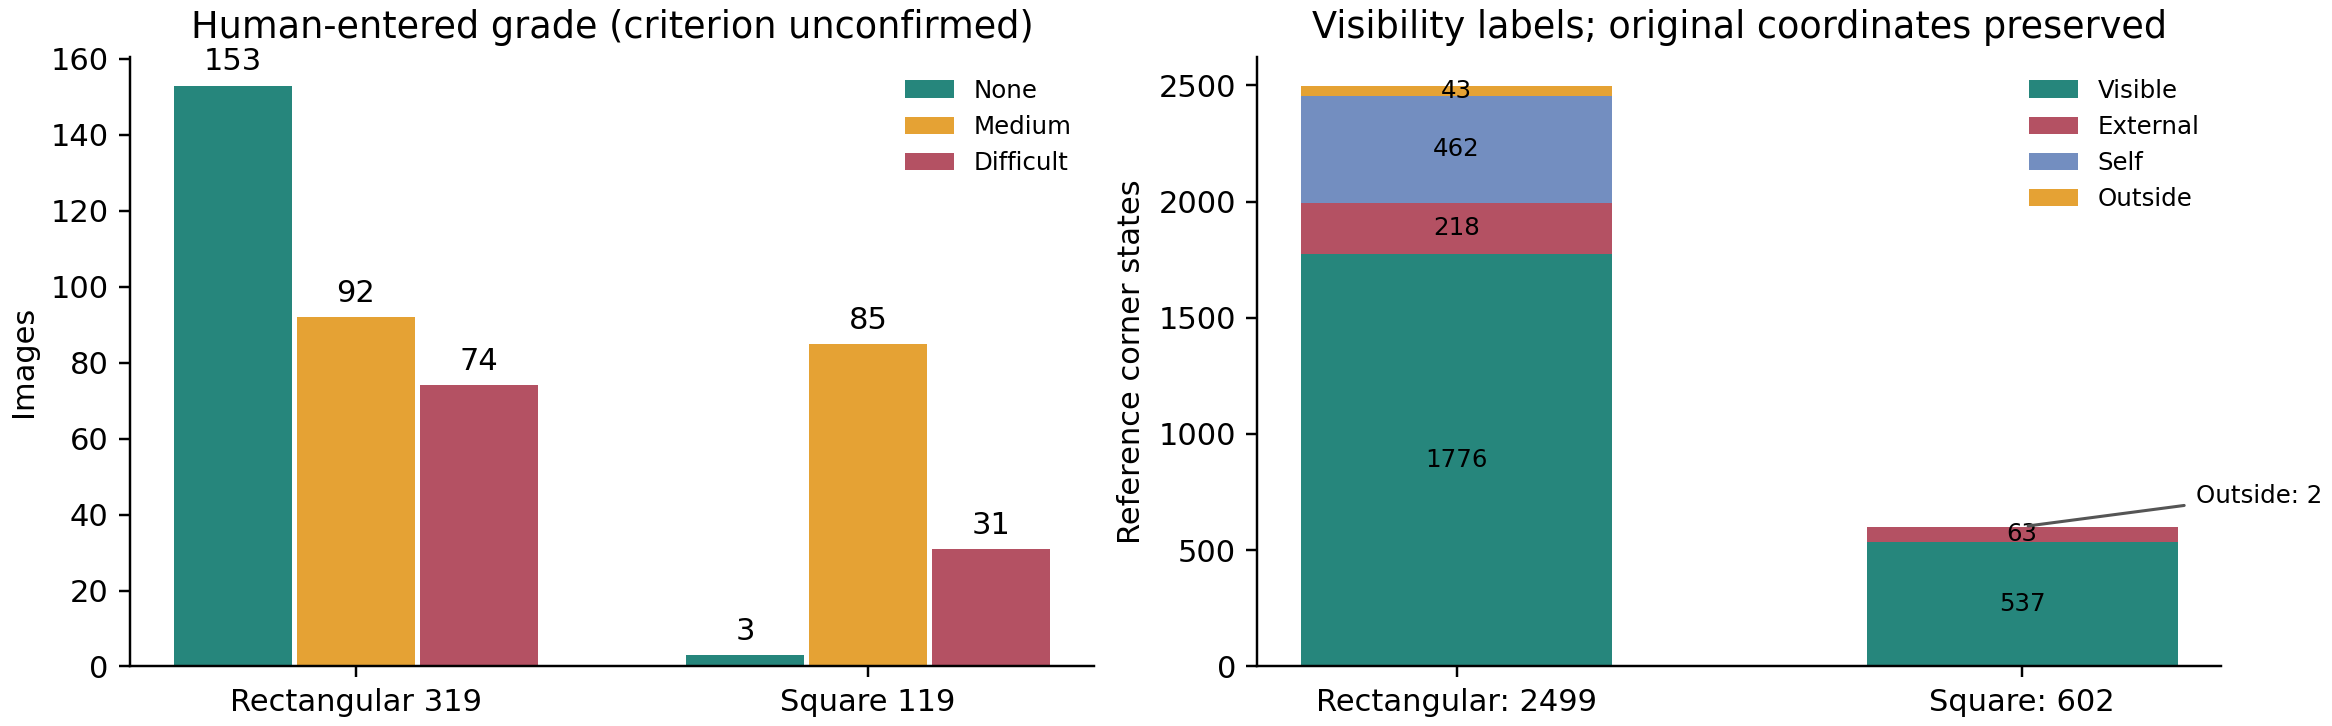
\includegraphics[width=.91\textwidth]{figures/current_review_summary.png}
\caption{최신 사람 입력의 자료 구성. 왼쪽 등급은 판정 기준 미확인 상태의 보조 분석이며, 오른쪽은 원래 참조 좌표를 유지한 가시성 상태다. 그림의 입력 개수는 모델 정확도나 독립 참조의 수가 아니다.}\label{sup:current_review_summary}
\end{figure*}


\section{큰 오류·손상·복구의 모든 집계}
표~\ref{sup:tail}은 본문에서 축약한 이동 상한 안팎의 개선·무차이·악화 개수를 보존한다. seed 1·2·3 각각의 개수이며 평균 개수를 실제 정수 표본처럼 표시하지 않는다. 유효 평가 코너는 2,445개, 2D 개선·6D 손상 공동 분석의 객체 매칭 영상은 311장이다. 전체 YOLO Base/N3 자세 통계와 산출은 319/319장으로 이 공동 분석 분모와 구분한다. 초기의 전체 참조 대응을 고정하고 같은 코너의 오차를 비교한다. 큰 오류를 줄이는 것과 10픽셀 미만으로 복구하는 것은 다른 관측이다.
% Generated from verified GitHub CSV at 7e136fc. See evidence/SOURCE_MANIFEST.json.
\begin{table*}[t]
\centering\footnotesize
\caption{동일 참조 대응을 고정한 큰 오류·손상·복구 분석. 각 칸은 seed 1 / 2 / 3의 실제 개수이다.}
\label{sup:tail}
\setlength{\tabcolsep}{3pt}
\begin{tabularx}{\textwidth}{Yrr}
\toprule
진단 항목 & Base → P & Base → N3 \\
\midrule
초기 오차가 이동 한계 이내 & 1,464 / 1,464 / 1,464 & 1,464 / 1,464 / 1,464 \\
초기 오차가 이동 한계 밖 & 981 / 981 / 981 & 981 / 981 / 981 \\
한계 안: 개선 & 882 / 886 / 883 & 954 / 936 / 908 \\
한계 안: 무차이 & 0 / 0 / 0 & 0 / 0 / 0 \\
한계 안: 악화 & 582 / 578 / 581 & 510 / 528 / 556 \\
한계 밖: 개선 & 686 / 668 / 690 & 720 / 716 / 725 \\
한계 밖: 무차이 & 0 / 0 / 0 & 0 / 0 / 0 \\
한계 밖: 악화 & 295 / 313 / 291 & 261 / 265 / 256 \\
양호($<5$px)$\to$악화($>10$px) & 0 / 1 / 0 & 0 / 0 / 1 \\
큰 오차($>20$px)$\to$복구($<10$px) & 0 / 0 / 0 & 0 / 2 / 0 \\
2D·이동·회전 모두 개선 (영상) & 114 / 113 / 112 & 126 / 129 / 124 \\
2D 개선, 이동 또는 회전 악화 (영상) & 138 / 140 / 138 & 147 / 129 / 141 \\
\bottomrule
\end{tabularx}
\tabnote{보정 범위는 원본 영상 대각선의 1\%이다. 코너 집계는 2,445점, 공동 변화 분석은 매칭된 311장이다. 마지막 두 행만 영상 수이고 그 위는 코너 수이다. 대칭 평가의 최적 대응 변경으로 이동 한계의 기하적 하한을 바꾸지 않았다. 무차이·악화·복구 없음도 그대로 보고한다.}
\end{table*}


\section{세션 구간과 seed 편차}
표~\ref{sup:pose_uncertainty}의 변화는 통계량(N3)−통계량(Base)이며 프레임별 차이의 중앙값이 아니다. 13세션을 단위로 동일한 10,000개 재표집을 만들고 각 재표집 안에서 세 seed의 통계 차이를 평균한다. 2.5·97.5백분위 구간과 seed 표준편차·최솟값·최댓값을 함께 제시한다. P90에서 악화하거나 0을 포함하는 구간도 보존한다. 이 구간은 반복 개발자료의 사후 분석으로 선택 편향·다중비교를 모두 보정한 독립 확증이 아니다.
% Generated from verified GitHub CSV at 7e136fc. See evidence/SOURCE_MANIFEST.json.
\begin{table*}[t]
\centering\footnotesize
\caption{N3−Base 자세 통계 차이의 사후 불확실성. 음의 차이는 오차 감소를 뜻한다.}
\label{sup:pose_uncertainty}
\setlength{\tabcolsep}{3pt}
\begin{tabularx}{\textwidth}{lYrrrr}
\toprule
기반 & 지표 & 평균 차이 & 95\% 구간 & seed 표준편차 & seed 최솟값 / 최댓값 \\
\midrule
YOLO & 이동 중앙값 (cm) & -0.829 & [-1.653, -0.195] & 0.293 & [-1.107, -0.523] \\
 & 이동 P90 (cm) & -2.721 & [-20.493, 5.710] & 0.367 & [-3.118, -2.394] \\
 & 회전 중앙값 (도) & -0.468 & [-0.886, -0.092] & 0.041 & [-0.511, -0.429] \\
 & 회전 P90 (도) & -0.608 & [-9.538, -0.071] & 0.037 & [-0.650, -0.577] \\
 & 방향각 중앙값 (도) & -0.182 & [-0.607, -0.052] & 0.025 & [-0.210, -0.162] \\
 & 방향각 P90 (도) & -0.571 & [-18.475, 0.132] & 0.056 & [-0.616, -0.508] \\
\midrule
DOPE & 이동 중앙값 (cm) & -1.690 & [-2.796, -0.786] & 0.087 & [-1.773, -1.599] \\
 & 이동 P90 (cm) & -4.739 & [-19.564, 4.923] & 1.016 & [-5.829, -3.818] \\
 & 회전 중앙값 (도) & -0.479 & [-0.893, -0.196] & 0.111 & [-0.605, -0.394] \\
 & 회전 P90 (도) & 1.590 & [-1.659, 7.847] & 0.881 & [0.573, 2.118] \\
 & 방향각 중앙값 (도) & -0.483 & [-0.667, 0.007] & 0.039 & [-0.528, -0.455] \\
 & 방향각 P90 (도) & 1.645 & [-1.664, 7.780] & 0.995 & [0.496, 2.233] \\
\midrule
ResNet-18$^{\dagger}$ & 이동 중앙값 (cm) & -0.604 & [-2.077, 0.202] & 0.071 & [-0.670, -0.529] \\
 & 이동 P90 (cm) & 2.759 & [-20.988, 3.960] & 0.695 & [2.091, 3.479] \\
 & 회전 중앙값 (도) & -0.510 & [-0.714, -0.022] & 0.064 & [-0.558, -0.437] \\
 & 회전 P90 (도) & 0.061 & [-0.520, 0.432] & 0.069 & [-0.019, 0.109] \\
 & 방향각 중앙값 (도) & -0.156 & [-0.361, 0.194] & 0.060 & [-0.198, -0.088] \\
 & 방향각 P90 (도) & 0.143 & [-0.533, 0.346] & 0.024 & [0.123, 0.170] \\
\bottomrule
\end{tabularx}
\tabnote{13개 촬영 세션을 단위로 동일한 10,000회 짝지은 재표집을 사용하고 각 재표집 안에서 세 seed의 통계 차이를 평균했다. 초기 난수 seed는 20260917이며 다중비교 보정은 없다. 통계량(after)−통계량(before)이지 프레임 차이의 중앙값이 아니다. ResNet 이동 중앙값처럼 구간이 0을 포함하는 결과를 확증적 개선으로 바꾸지 않는다.}
\end{table*}


\section{처리 시간의 상세 계측}
표~\ref{sup:cost}는 전체 CUDA event 중앙값·P90, 동기화 벽시계 중앙값, 보정 단독 시간과 최대 할당 메모리이다. 전체 중앙값 차이와 보정 단독 중앙값은 다른 계측량이다. 26프레임·batch 1·seed 1·준비 20회·프레임당 5반복을 사용하며 파일 읽기는 제외한다. DOPE·ResNet과 YOLO는 같은 GPU지만 실행환경이 달라 별도 패널로 표시한다. 이전 표는 다른 보정기 전체를 동일 환경에서 측정한 효율 순위를 뜻하지 않는다. 본문에 추가한 Base/N3/PoseFix 공정 계측은 별도 RUNTIME\_MATCHED/VERIFICATION 영수증의 벽시계 경계를 사용한다.
% Generated from verified GitHub CSV at 7e136fc. See evidence/SOURCE_MANIFEST.json.
\begin{table*}[t]
\centering\footnotesize
\caption{고정 26프레임·seed 1의 처리 시간과 추가 파라미터. 같은 RTX 3080에서 실행 환경을 분리하여 표시하였다.}
\label{sup:cost}
\setlength{\tabcolsep}{2.5pt}
\begin{tabularx}{\textwidth}{Yrrrrrr}
\toprule
기반·경로 & 추가 파라미터 & 전체 중앙(ms) & 전체 P90(ms) & 벽시계 중앙(ms) & 보정 중앙(ms) & 최대 메모리(MiB) \\
\midrule
\multicolumn{7}{l}{\textbf{환경: pallet-yolo26}} \\
YOLO Base & 0 & 11.195 & 13.712 & 11.237 & \NA & 62.24 \\
YOLO N3 & 20,259 & 15.138 & 17.212 & 15.179 & 3.432 & 64.52 \\
\midrule
\multicolumn{7}{l}{\textbf{환경: pallet-pose}} \\
DOPE Base & 0 & 62.736 & 77.585 & 62.779 & \NA & 342.39 \\
DOPE N3 & 23,331 & 65.807 & 80.927 & 65.838 & 2.838 & 342.39 \\
ResNet-18$^{\dagger}$ Base & 0 & 8.890 & 9.573 & 8.933 & \NA & 98.85 \\
ResNet-18$^{\dagger}$ N3 & 23,331 & 11.592 & 12.747 & 11.632 & 2.632 & 98.85 \\
\bottomrule
\end{tabularx}
\tabnote{경로별 준비 20회와 프레임당 5반복, 배치 1; 파일 읽기는 계측에서 제외한다. 전체 중앙/P90 및 보정 중앙은 CUDA event 시간이며 동기화 벽시계도 함께 남겼다. YOLO는 이번 추가 측정이고 DOPE·ResNet은 같은 고정 계약의 기존 측정이다. 환경 차이를 무시한 순수 하드웨어 비교 또는 Jetson 성능으로 해석하지 않는다. 보정 없는 경로의 보정 시간은 해당 없음이다.}
\end{table*}


\section{비교군의 정보와 확인되지 않은 항목}
표~\ref{sup:comparator_contract}는 결과 차이 해석에 필요한 입력·학습 범위를 정리한다. 확인되지 않은 사전학습·선택 이력을 동일하다고 가정하지 않는다. 보정 의사 레이블 학생의 교사는 별도 실사 감독과 구조를 사용하므로 N3 교사로 부르지 않는다. 원 논문의 결과와 팔레트에 적용한 변형의 결과도 구분한다.
\begin{table*}[t]\centering\footnotesize
\caption{보정 비교군의 입력·학습 범위와 남은 확인.}\label{sup:comparator_contract}
\begin{tabularx}{\textwidth}{lYYY}\toprule
방법 & 입력·변화하는 부분 & 확인된 추가 학습 & 해석상 제한 \\\midrule
N3 & 내부 특징·초기 코너·박스·치수; 국소 코너 이동 & 3 seed, 6,000 updates, 96,000 노출/seed; 합성 calibration 온도 & 기반별 초기 학습·유효 표본은 다름 \\
P / D / L & 내부 특징 기반 보정; 분포/회귀/선 구조의 출력·손실 차이 & 동결된 기존 체크포인트, 3 seed 평가 & 각 방법의 전체 감독·사전학습·튜닝 명세 추가 확인; 같은 예산이라고 소급 가정하지 않음 \\
PoseFix 기반 & 영상·초기 자세; 팔레트 9점용 목표·지원 영역 변형 & 공식 네트워크 연산 대조; 3 seed, 6,000 updates, 96,000 노출/seed & 원 논문 전체 수렴 학습과 다름; 사전학습·자료·선택 경로의 완전한 동등성 미확인 \\
업데이트 학생 & 초기 추정기의 가중치 갱신 & 완료된 기존 학생을 공통 128장에 평가 & 별도 교사·감독 예산; 독립 TEST 아님 \\
\bottomrule\end{tabularx}
\end{table*}

\section{기록 영상의 시계열 출력}
본문의 사례는 같은 네 기록 영상 8,910프레임에 대한 고정 모델 오프라인 비교이다. 두 방법의 frame ID와 결측 마스크는 전수 일치했고, 각각 8,772개의 새 자세와 138개의 no-pose를 냈으며 held 출력은 없었다. 표~\ref{sup:lifter_sessions}는 세션별 저장 분모와 가용성을 보인다. 이 수치는 사람 참조가 없는 출력 연속성이다. 운용 모델의 출력이나 제어 명령을 정답으로 사용하지 않는다. 별도 12장의 원래 G 기하 참조 96좌표(직접 클릭 66점·PnP 투영 30점)와 이후 직접 클릭 72점·자체 가림 24상태의 버전을 구분하고, 실제 대상 대응 12건을 확보하였다. 원래 공식 120/24장 직접 가시 참조 계약과 정지·독립 물리 참조가 필요한 값은 x로 보존하며, 별도 기하 참조 오차는 다음 절에 제시한다.
\begin{table}[t]\centering\footnotesize
\caption{기록 영상 세션별 고정 출력 가용성. Base와 N3의 분모와 상태는 같다.}\label{sup:lifter_sessions}
\begin{tabularx}{\columnwidth}{Yrrrr}\toprule
세션 & 저장 & fresh/no-pose & 산출률(\%) & 최장 완료 결측(s) \\\midrule
173507 & 3,729 & 3,678/51 & 98.632 & 0.534 \\
174126 & 757 & 717/40 & 94.716 & 2.268 \\
174342 & 2,501 & 2,501/0 & 100.000 & NA \\
174925 & 1,923 & 1,876/47 & 97.556 & 2.535 \\
\bottomrule\end{tabularx}
\tabnote{최장 결측은 첫 no-pose 저장 프레임에서 다음 fresh 프레임까지의 센서 시간이다. 저장되지 않은 카메라 프레임은 모델 실패로 세지 않는다.}
\end{table}
\begin{figure}[t]\centering
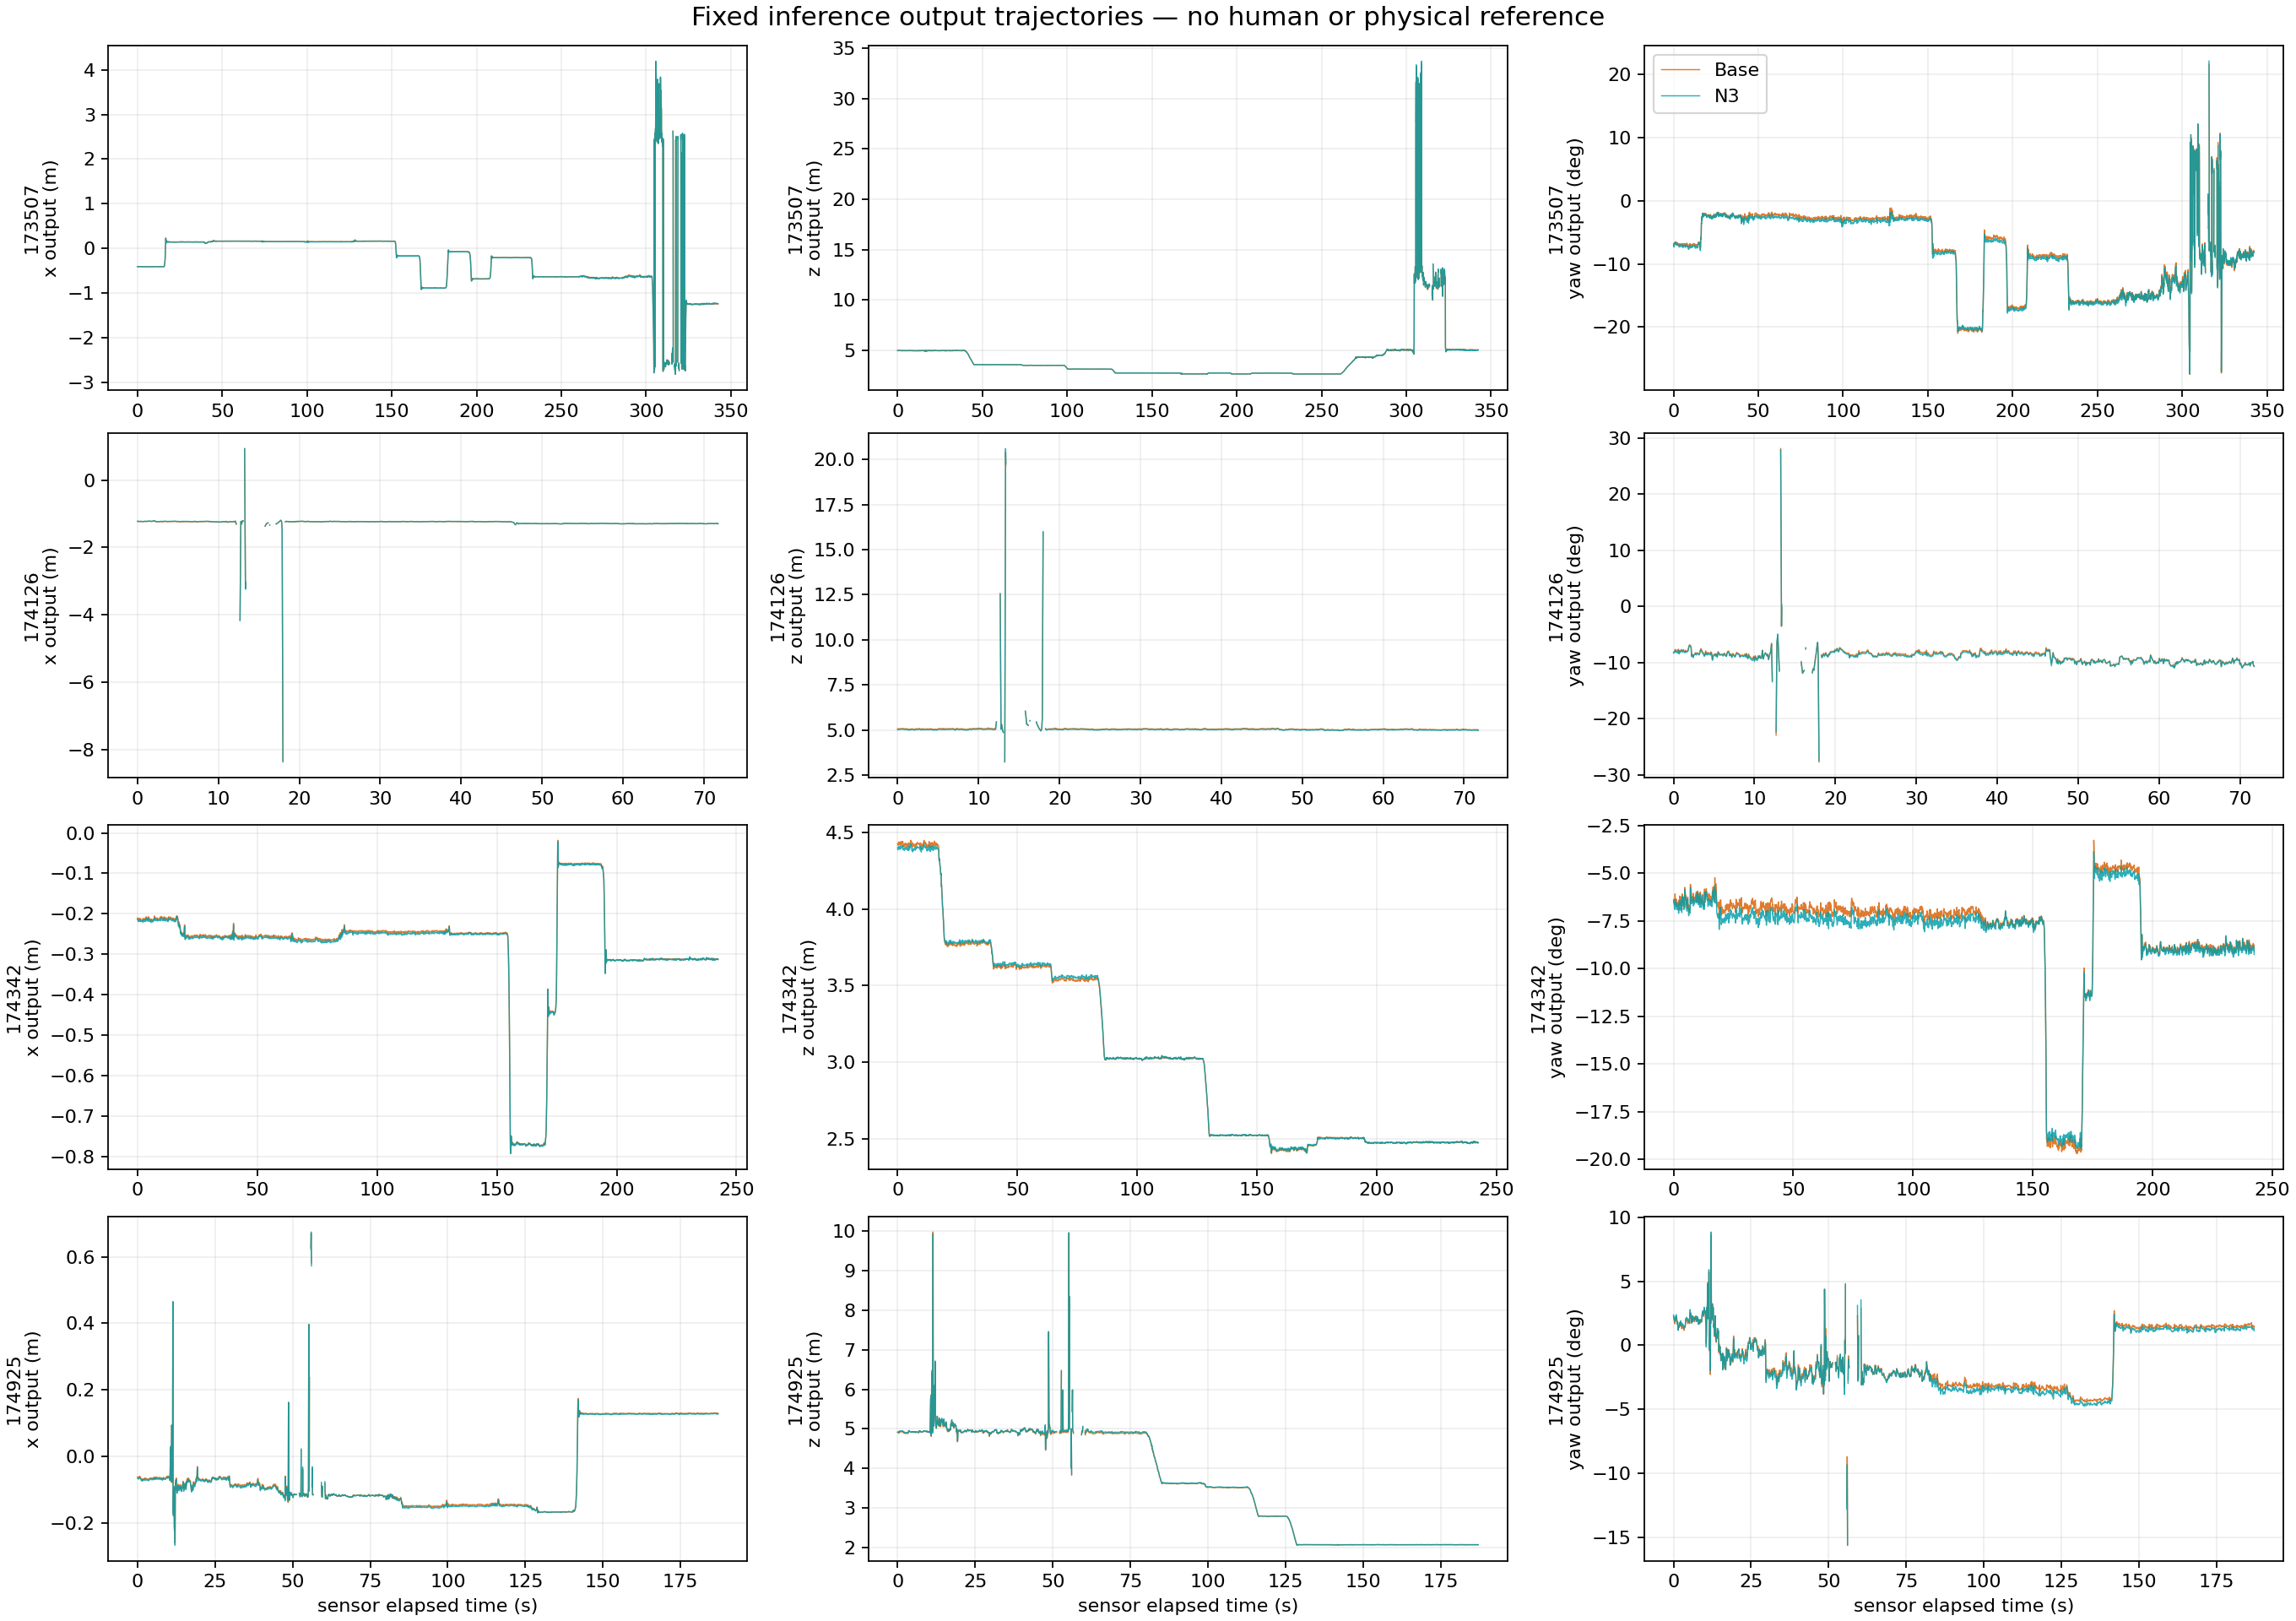
\includegraphics[width=\columnwidth]{figures/lifter_prediction_timeseries.png}
\caption{네 기록 영상의 Base와 Base+N3 자세 출력. 유한 출력만 연결하고 no-pose는 공백으로 남겼다. 정답 또는 실제 물리 궤적은 포함하지 않으므로 곡선의 근접성은 정확도 근거가 아니다.}\label{sup:case_slots}
\end{figure}

\section{PnP 보조 기하 참조의 별도 12장 탐색 패널}
별도 탐색 패널은 네 세션에서 사전에 고정한 12장의 원래 G 저장본 96좌표를 사용한다. 직접 클릭 66점과 알려진 기하·클릭을 이용한 PnP 투영 30점을 동일한 0–7 코너 대응으로 평가한다. 이후 가시성 재검수의 직접 클릭 72점·자체 가림 24상태는 별도 버전으로 보존하고 혼합하지 않는다. 사람이 고정 선택 박스를 검수한 12장 모두 실제 주석 대상과 같았으며, 두 방법에 같은 frame ID·코너·선택 인덱스·결측 마스크를 적용했다. 참조 좌표를 모델 출력으로 교체하지 않고 재-PnP·점별 최근접 대응·튜닝·추가 학습 없이 원시 예측만 재집계했다. 이 패널은 공식 120장/24장 반복 가시 코너 검수나 독립 물리 T/R 측정을 완료한 결과가 아니다.
\begin{table}[t]\centering\footnotesize
\caption{같은 12장 기하 참조 패널의 네 세션별 결과. 각 세션은 3장·24점이다.}\label{sup:lifter_assisted_sessions}
\begin{tabularx}{\columnwidth}{Ylrrrr}\toprule
세션 & 방법 & 중앙(px) & P90(px) & PCK(\%) & 유효/전체 \\\midrule
173507 & Base & 3.699 & 11.772 & 79.167 & 24/24 \\
173507 & N3 & 3.786 & 10.390 & 87.500 & 24/24 \\
174126 & Base & 4.349 & 9.540 & 91.667 & 24/24 \\
174126 & N3 & 5.434 & 8.794 & 95.833 & 24/24 \\
174342 & Base & 3.999 & 8.339 & 100.000 & 24/24 \\
174342 & N3 & 3.811 & 7.641 & 100.000 & 24/24 \\
174925 & Base & 4.306 & 9.473 & 95.833 & 24/24 \\
174925 & N3 & 4.158 & 9.198 & 95.833 & 24/24 \\
\bottomrule\end{tabularx}
\tabnote{고정 YOLO Base와 N3(seed 1)의 원시 예측을 재사용하였다. 중앙값/P90은 조건부 통계이고 PCK 분모에는 결측과 대상 불일치를 유지한다. 이 표에서는 두 방법 모두 96점이 유효하며 실패는 0점이다. 네 세션의 모든 고정 표본을 보존했다. 3 seed 평균이나 8,910프레임의 참조 정확도가 아니다.}
\end{table}


같은 코너 96점에서 통계량 차이 median(N3)−median(Base)는 0.210px, P90(N3)−P90(Base)는 −0.666px이고, 점별 차이의 중앙값 median(N3−Base)는 0.090px다. 서로 다른 통계량을 혼동하지 않았다. 점별 개선/악화/동일은 46/50/0점이며, 프레임별 코너 중앙값의 변화는 개선 5장·악화 7장이다. PCK 적중은 88→91점으로 3.125\%p 증가했다. 원래 G 참조 생성 시점의 독립 블라인드 이력은 확인되지 않았으며, 현재 선택 박스 확인 이력은 실제 사람 검수 기록에 구분해 저장했다. 직접 클릭과 투영은 참조의 출처 정보이며 그 구분만으로 투영점을 배제하거나 수동 클릭의 우월성을 가정하지 않았다.
\begin{figure*}[t]\centering
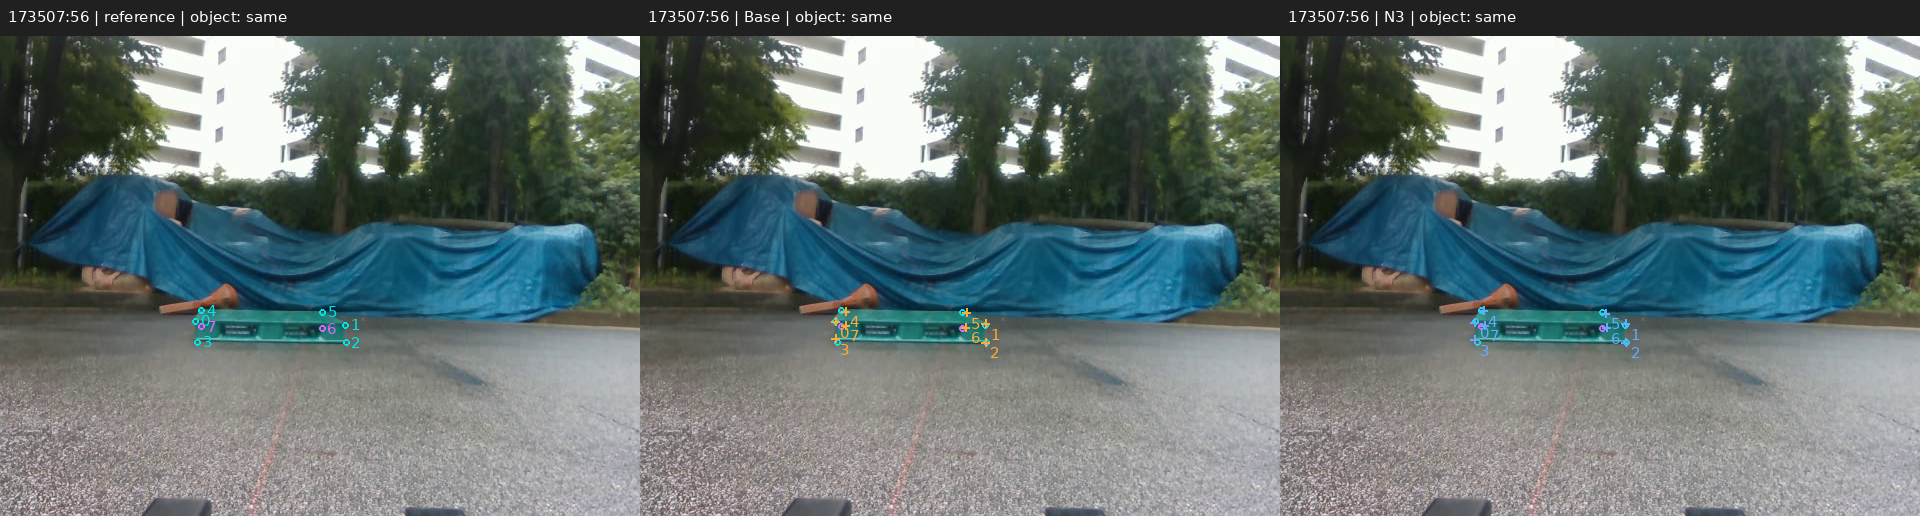
\includegraphics[width=.97\textwidth]{figures/pnp_assisted_lifter_12/173507_56.png}\par\smallskip
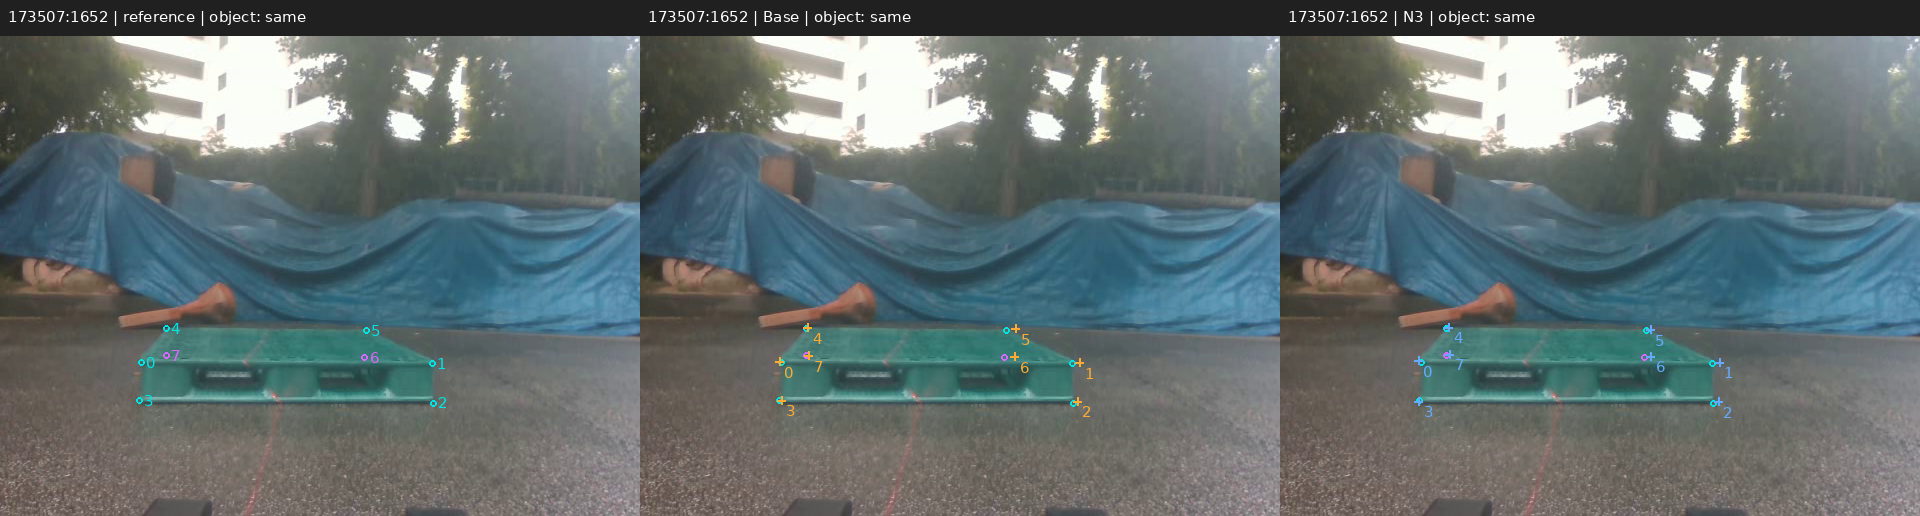
\includegraphics[width=.97\textwidth]{figures/pnp_assisted_lifter_12/173507_1652.png}\par\smallskip
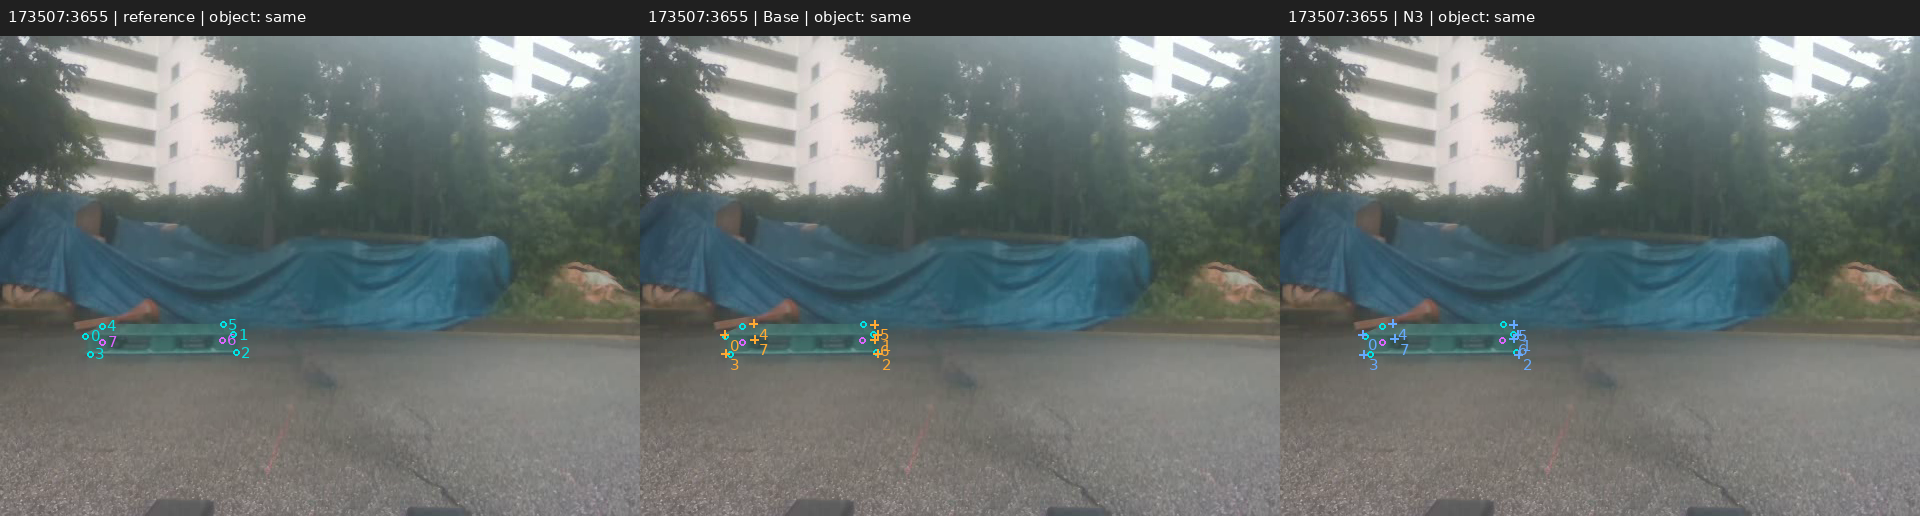
\includegraphics[width=.97\textwidth]{figures/pnp_assisted_lifter_12/173507_3655.png}\par\smallskip
\caption{173507세션의 사전 고정 3장 전체. 왼쪽은 원래 기하 참조(청록 직접 클릭·보라 PnP), 가운데 Base, 오른쪽 N3이다. 생성 경로를 표시하며 독립 물리 정답이나 모든 점의 직접 가시성을 뜻하지 않는다.}\label{sup:lifter_assisted_173507}
\end{figure*}
\begin{figure*}[t]\centering
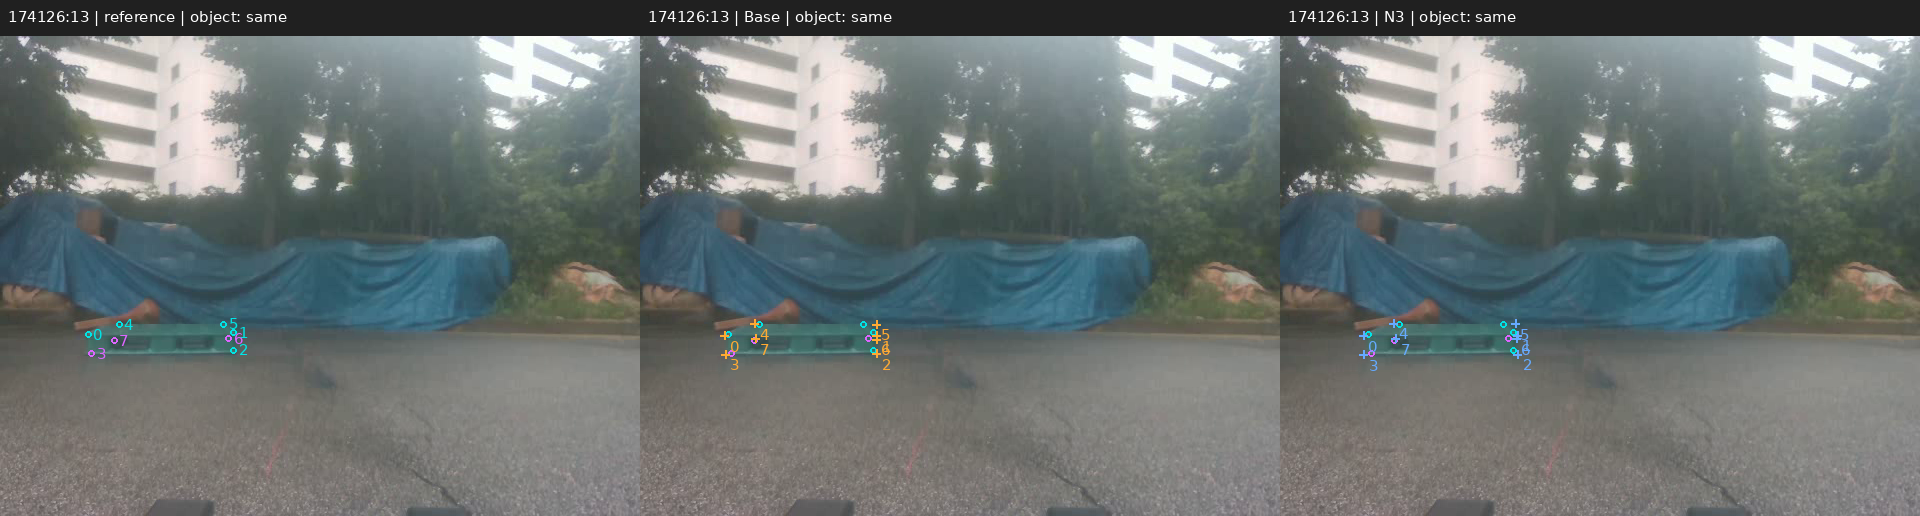
\includegraphics[width=.97\textwidth]{figures/pnp_assisted_lifter_12/174126_13.png}\par\smallskip
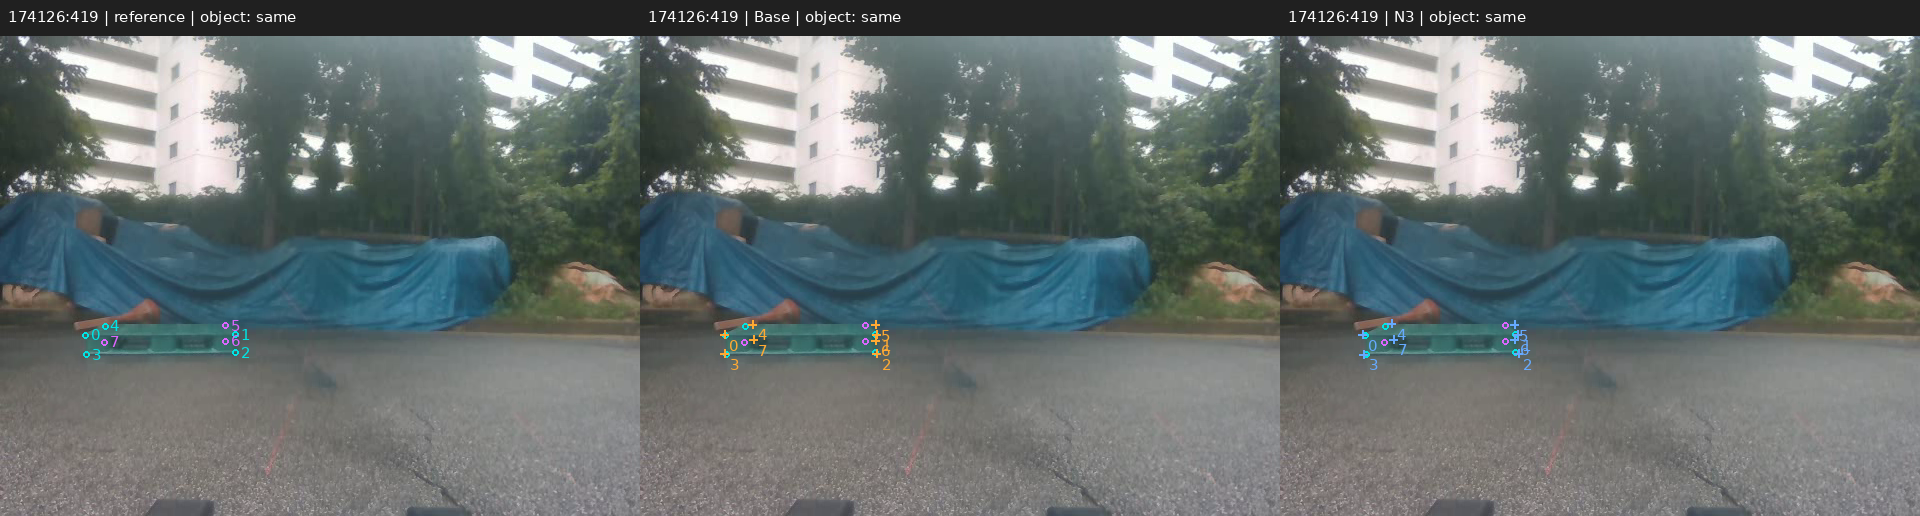
\includegraphics[width=.97\textwidth]{figures/pnp_assisted_lifter_12/174126_419.png}\par\smallskip
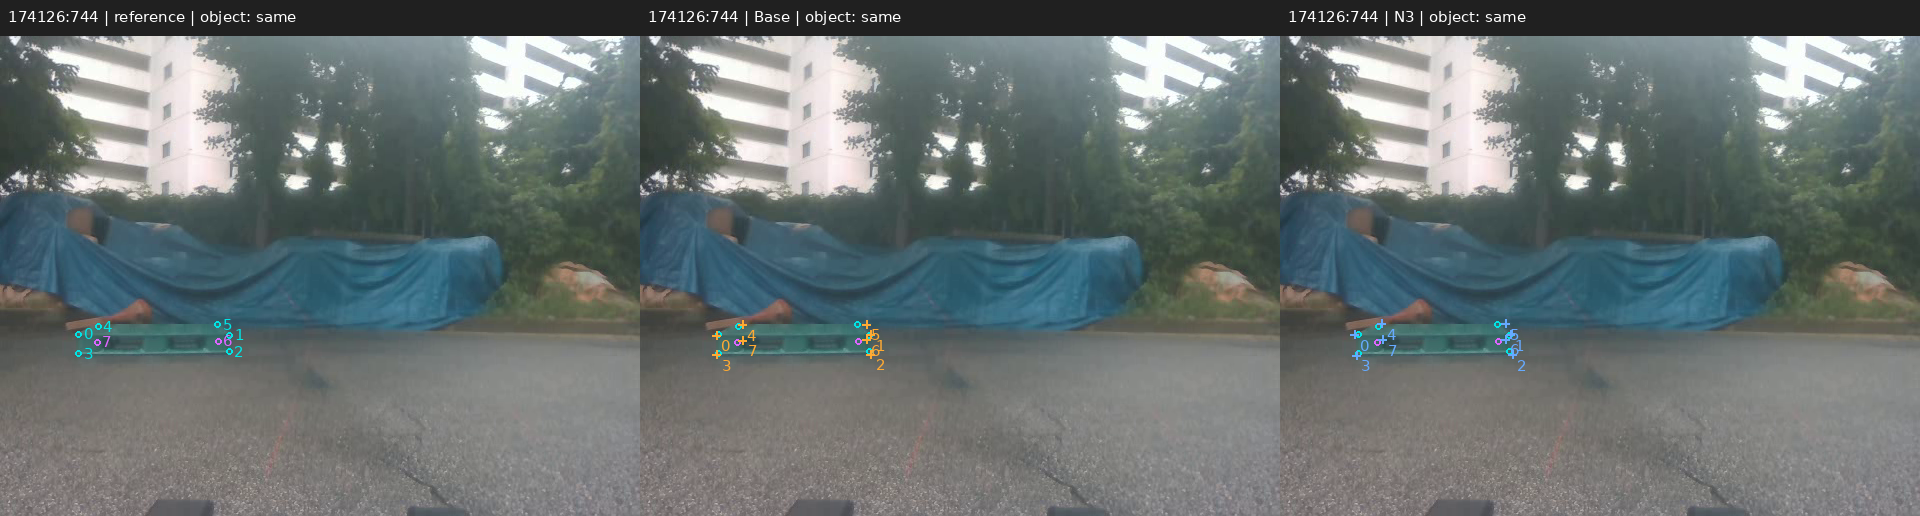
\includegraphics[width=.97\textwidth]{figures/pnp_assisted_lifter_12/174126_744.png}\par\smallskip
\caption{174126세션의 사전 고정 3장 전체. 왼쪽은 원래 기하 참조(청록 직접 클릭·보라 PnP), 가운데 Base, 오른쪽 N3이다. 생성 경로를 표시하며 독립 물리 정답이나 모든 점의 직접 가시성을 뜻하지 않는다.}\label{sup:lifter_assisted_174126}
\end{figure*}
\begin{figure*}[t]\centering
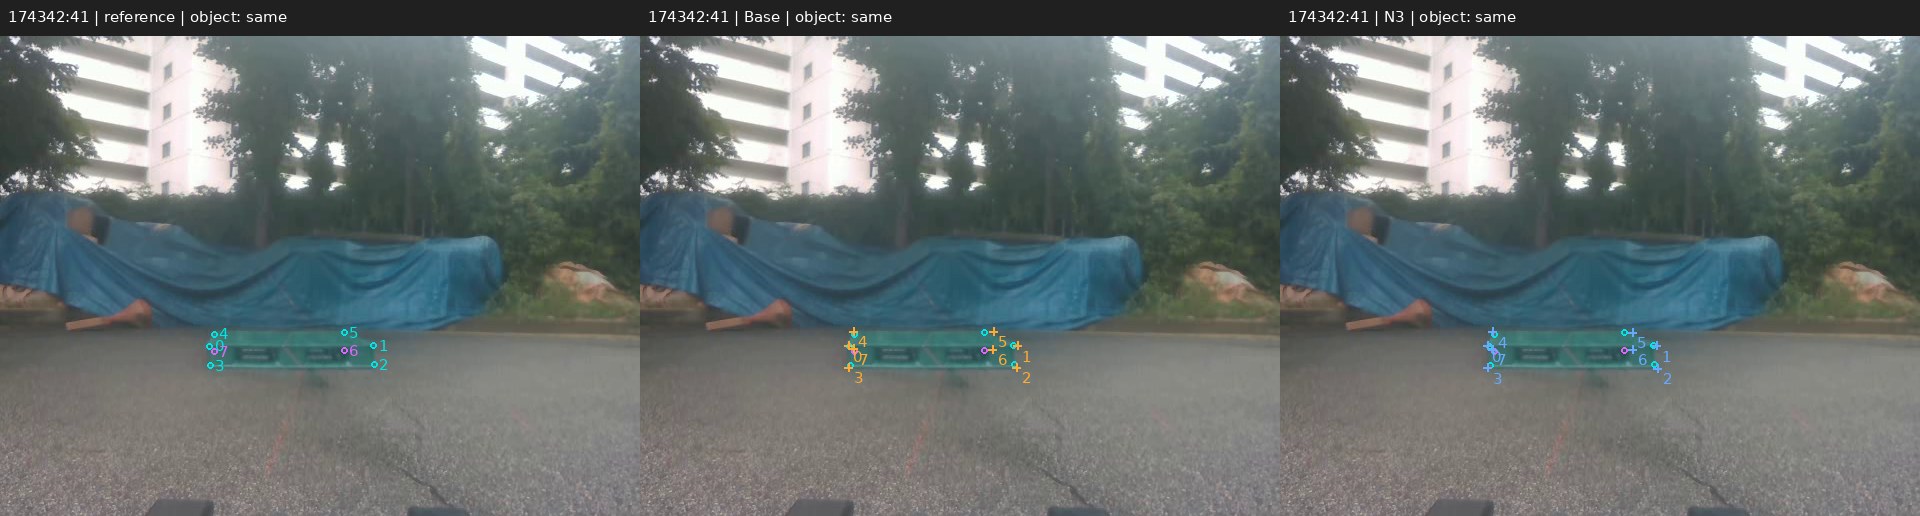
\includegraphics[width=.97\textwidth]{figures/pnp_assisted_lifter_12/174342_41.png}\par\smallskip
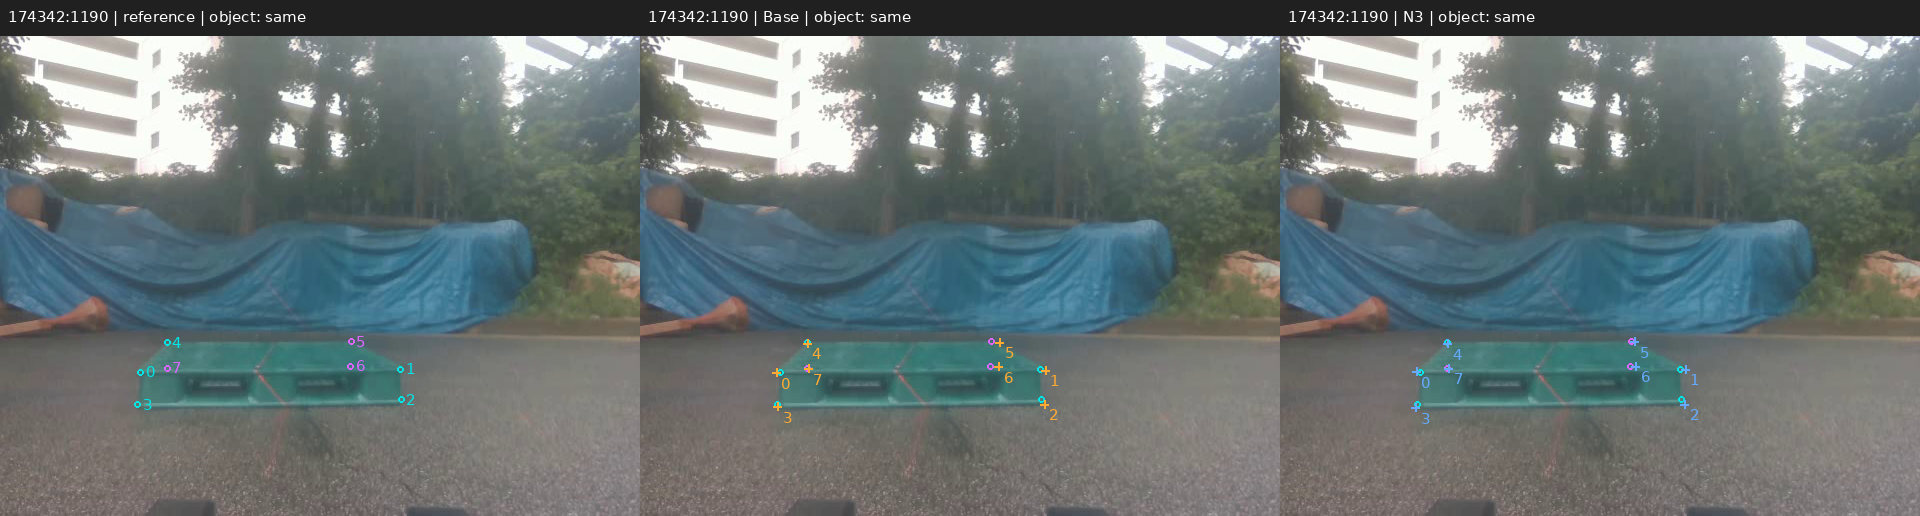
\includegraphics[width=.97\textwidth]{figures/pnp_assisted_lifter_12/174342_1190.png}\par\smallskip
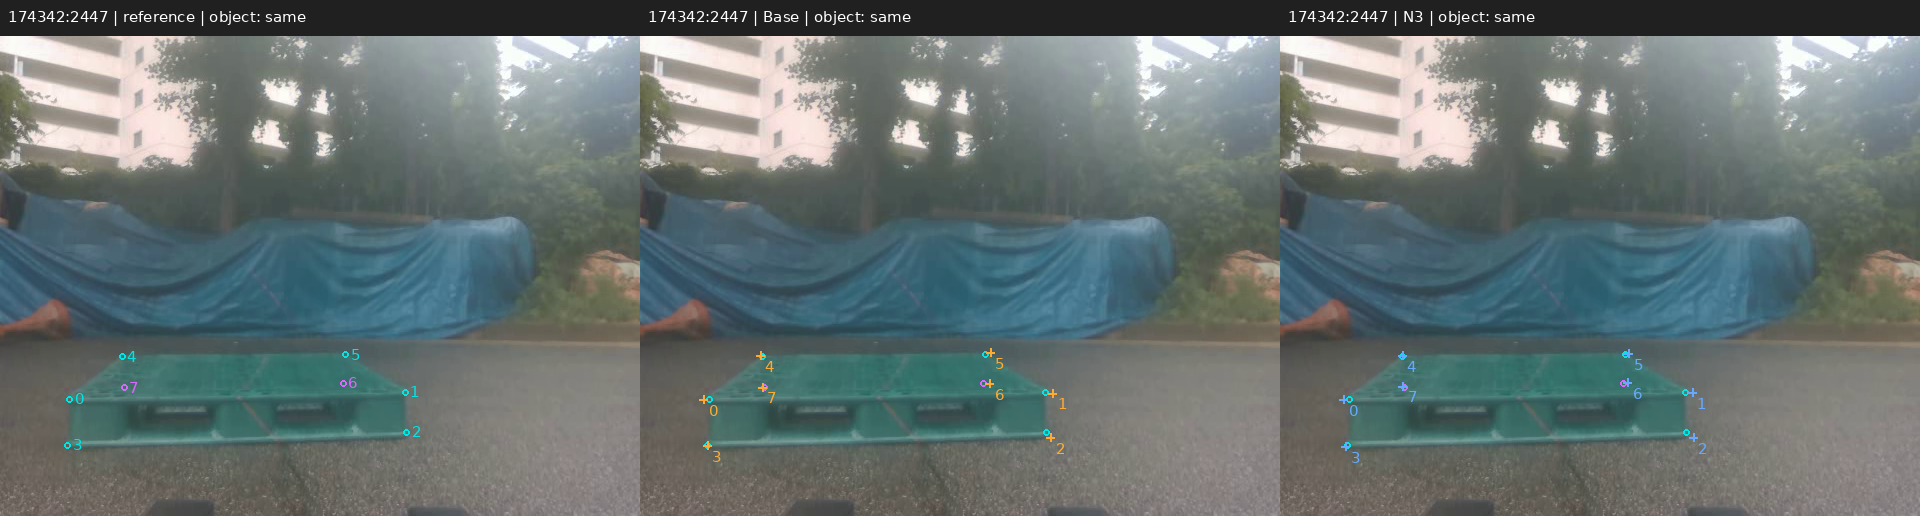
\includegraphics[width=.97\textwidth]{figures/pnp_assisted_lifter_12/174342_2447.png}\par\smallskip
\caption{174342세션의 사전 고정 3장 전체. 왼쪽은 원래 기하 참조(청록 직접 클릭·보라 PnP), 가운데 Base, 오른쪽 N3이다. 생성 경로를 표시하며 독립 물리 정답이나 모든 점의 직접 가시성을 뜻하지 않는다.}\label{sup:lifter_assisted_174342}
\end{figure*}
\begin{figure*}[t]\centering
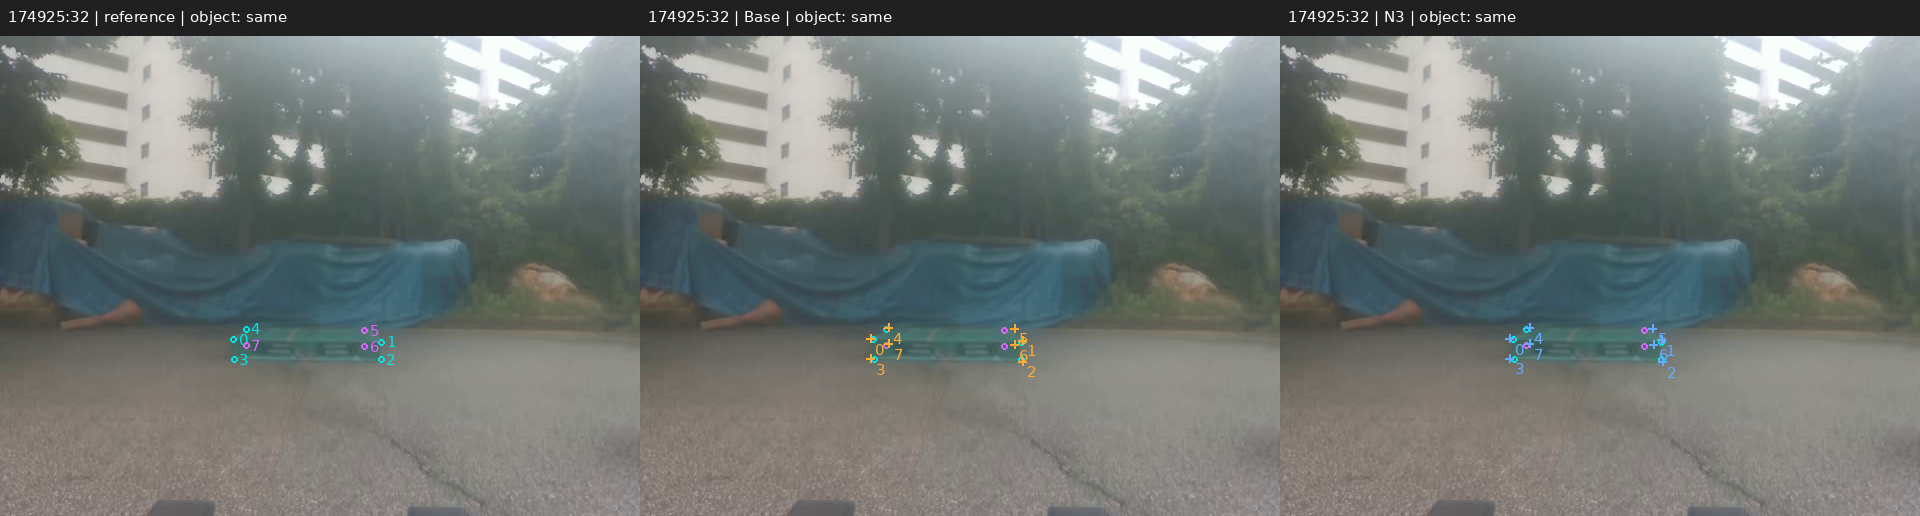
\includegraphics[width=.97\textwidth]{figures/pnp_assisted_lifter_12/174925_32.png}\par\smallskip
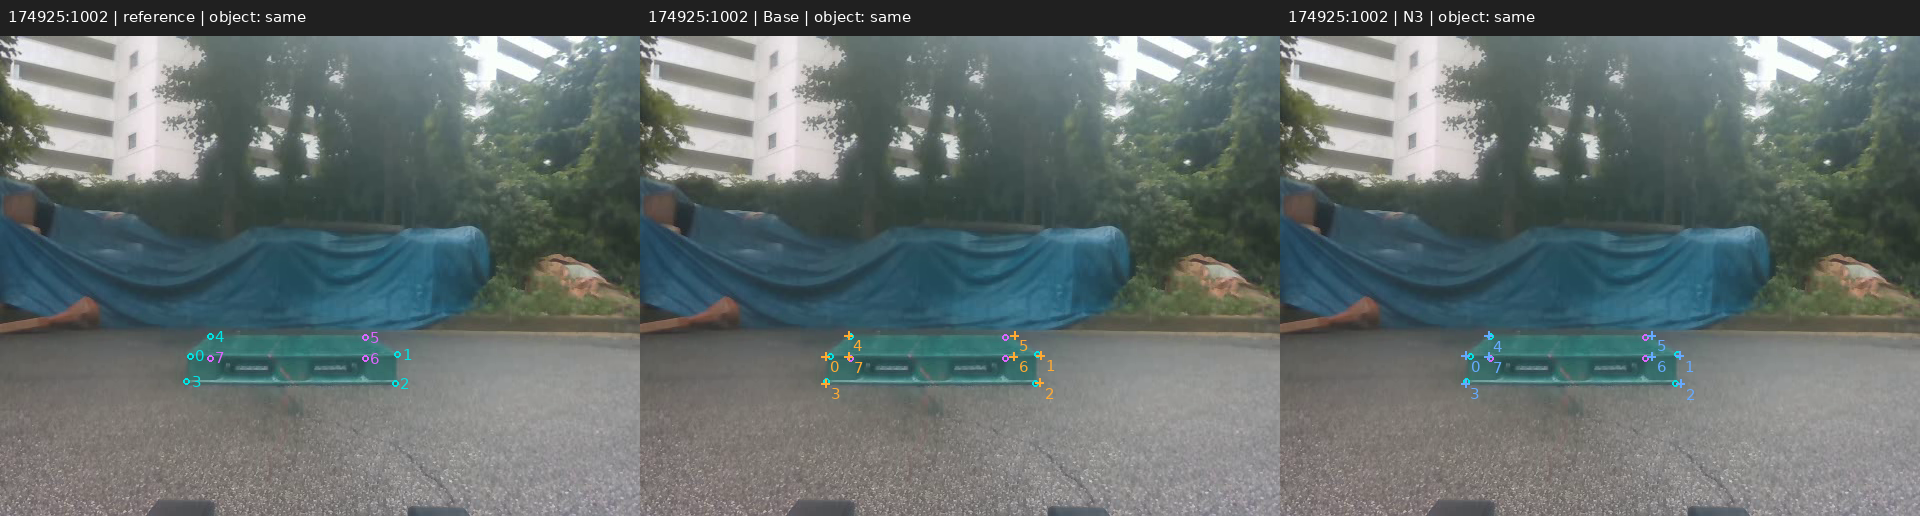
\includegraphics[width=.97\textwidth]{figures/pnp_assisted_lifter_12/174925_1002.png}\par\smallskip
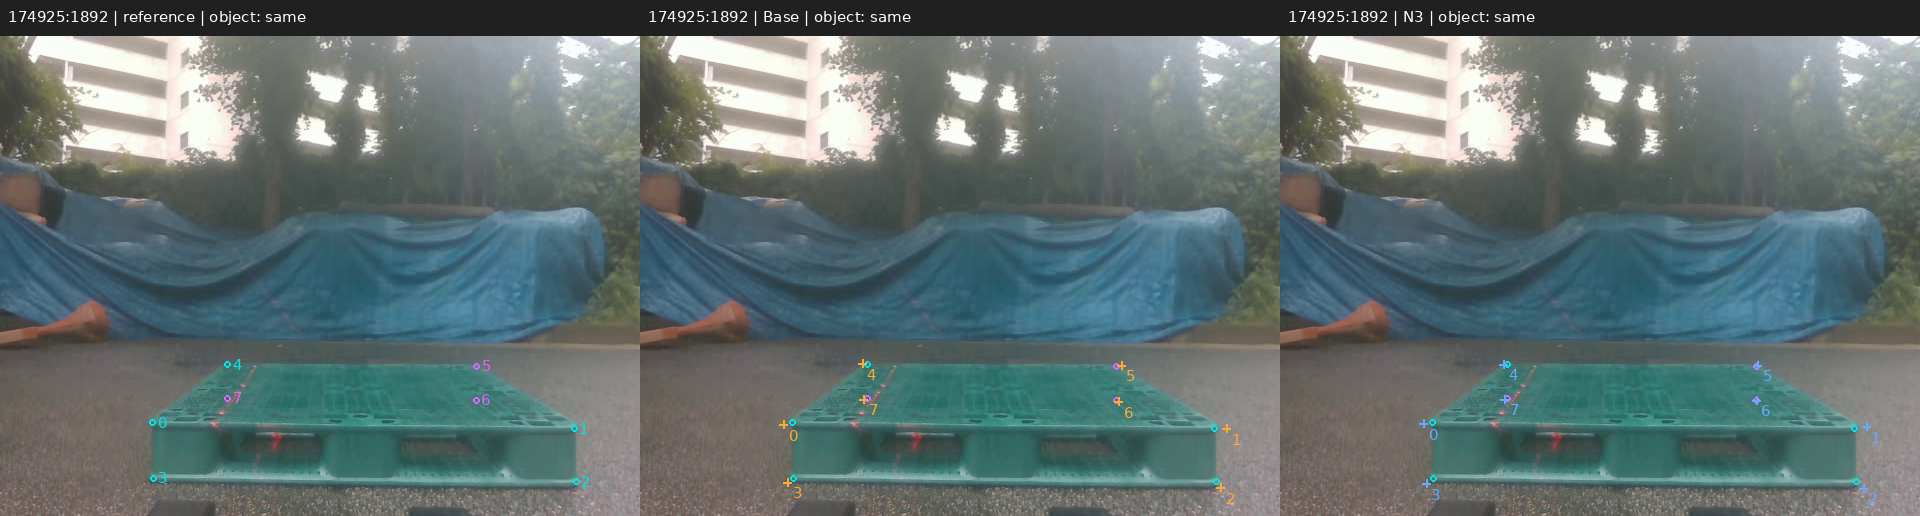
\includegraphics[width=.97\textwidth]{figures/pnp_assisted_lifter_12/174925_1892.png}\par\smallskip
\caption{174925세션의 사전 고정 3장 전체. 왼쪽은 원래 기하 참조(청록 직접 클릭·보라 PnP), 가운데 Base, 오른쪽 N3이다. 생성 경로를 표시하며 독립 물리 정답이나 모든 점의 직접 가시성을 뜻하지 않는다.}\label{sup:lifter_assisted_174925}
\end{figure*}

\FloatBarrier

\section{추가 인계 자료와 기존 결과의 연결 검산}
원래 검수 계획은 주 120건과 같은 사진의 반복 24건으로, 고유 사진 120장이다. 실제 사용자 제외 기록은 주 5건·반복 1건이며 제외 사진을 재투입하지 않았다. 기존 12장의 탐색적 기하 참조를 주 기록에 재사용할 수 있고, 미확보 주 참조 103건·실제 반복 기록 23건은 따로 남긴다. 이 원장 집계는 공식 전체 가시 코너 정확도나 반복 품질의 완료가 아니다. 원계획의 분모를 소급 변경하거나 주 좌표를 반복 주석으로 복사하지 않았다. 추가 클릭을 새로 요구하지 않았으며, 승인 미제출인 후속 좌표 저장본의 버전 민감도는 아래에 별도로 제시한다.
\begin{table}[t]\centering\footnotesize
\caption{추가 인계 자료와 수신 측 기존 결과의 연결 검산. 정확도 표가 아니다.}\label{sup:remaining_connection}
\begin{tabularx}{\columnwidth}{Yrr}\toprule
항목 & 분모 & 확인 수 \\\midrule
원영상 픽셀·시각 연결 & 8,910 & 8,910 \\
보존한 중복 관측 & 8,910 & 29 \\
정사각형 원사진·주석 & 119 & 119 \\
기존 full 6D 예측 / 방법 & 8,910 & 8,772 \\
독립 물리 참조 연결 & 9,029 & 0 \\
\bottomrule\end{tabularx}
\end{table}

\subsection{중립 명령 조건의 저장 출력}
모델 출력을 보지 않고 명령 기록에서 정의한 모든 32개 중립 CAN 구간을 재사용하였다. 센서 시각으로 연결한 저장 프레임은 8,263개이며 Base와 N3 각각 fresh 8,125개, no-pose 138개, held 0개이다. 동일 구간 안에서 x/z의 모집단 표준편차와 360도 wrapping만 제거한 yaw 표준편차를 계산했고 90/180도 가지 변화와 결측을 남겼다. 이는 명령 조건의 출력 분산이며 물리 정지·정착·잡음·정확도를 증명하지 않는다. 구간을 낮은 분산 순으로 고르거나 이동 구간을 제거하지 않았다. 실제 상대 정지 승인과 사전 선정 이력의 근거가 없어 원래 정지 evaluator의 x는 유지한다.
\begin{table}[t]\centering\footnotesize
\caption{중립 명령 32구간의 출력 가용성. 상대 정지 미확인 사후 기술 패널.}\label{sup:command_intervals}
\begin{tabularx}{\columnwidth}{Yrr}\toprule
항목 & Base & N3 \\\midrule
저장 프레임 & 8,263 & 8,263 \\
fresh & 8,125 & 8,125 \\
no-pose & 138 & 138 \\
held & 0 & 0 \\
정지 잡음 & \notrun & \notrun \\
\bottomrule\end{tabularx}
\end{table}

\begin{figure}[t]\centering
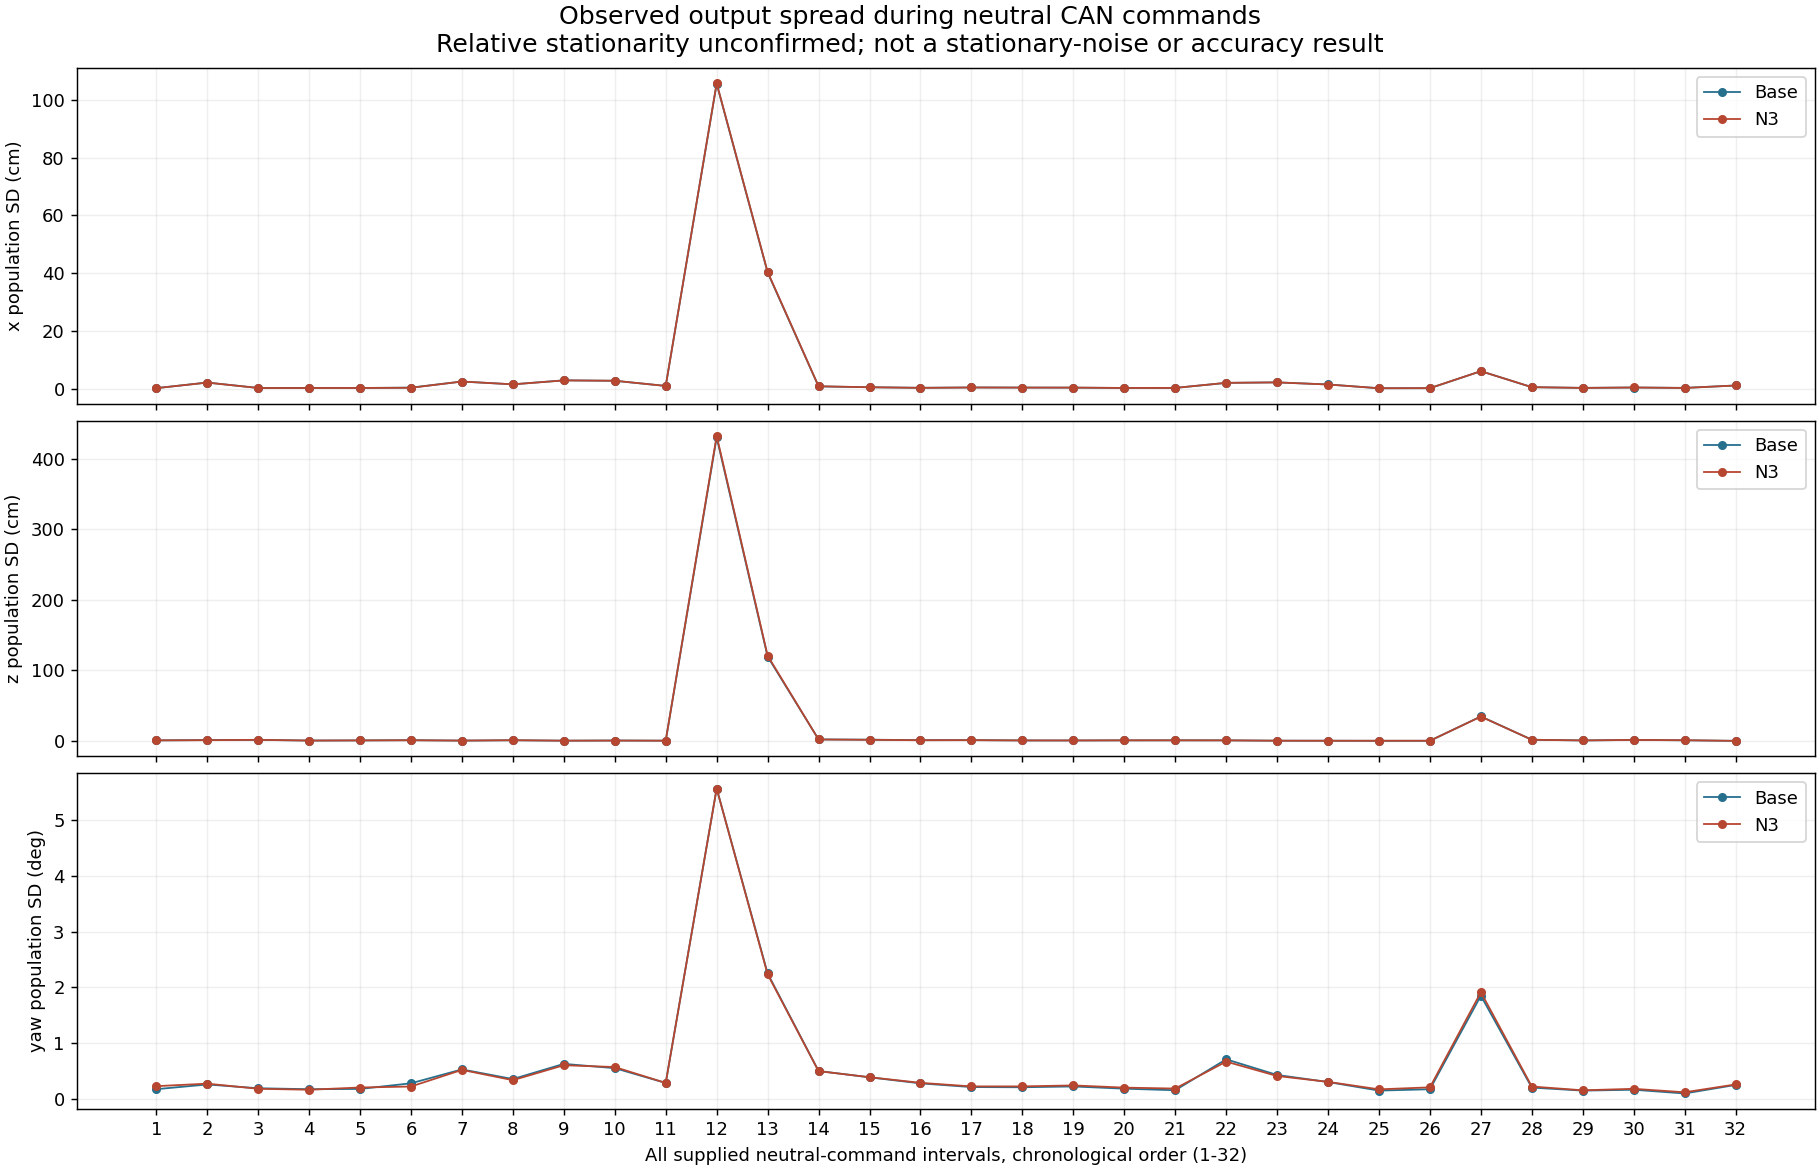
\includegraphics[width=\columnwidth]{figures/all_32_command_spreads.png}
\caption{모든 중립 명령 후보의 구간별 출력 분산. 실제 상대 정지 미확인으로 정지 잡음이 아니다.}\label{sup:neutral_command_spread}
\end{figure}
\subsection{후속 좌표 저장본의 참조 버전 민감도}
후속 저장본의 같은 12장·72좌표만을 고정하여 참조 버전 민감도를 확인하였다. 기존 직접 클릭 66좌표는 정확히 같고 원래 PnP였던 6자리에는 실제 나중 저장 좌표가 존재한다. 나머지 자체 가림 24자리는 좌표를 새로 생성하지 않았다. 저장본은 승인 미제출 초안이며 evaluation\_use=false이므로 이 결과를 공식 직접 가시 참조 정확도라고 주장하지 않는다. 원래 96점 결과를 교체하거나 오차를 보고 참조 버전을 선택하지 않았으며 각 표의 분모를 구분하였다.
\begin{table}[t]\centering\footnotesize
\caption{미제출 후속 저장본의 참조 버전 민감도(12장·72좌표). 공식 정확도와 별도.}\label{sup:reference_version_sensitivity}
\begin{tabularx}{\columnwidth}{Yrrrr}\toprule
방법 & 중앙 px & P90 px & PCK(\%) & 유효/전체 \\\midrule
Base & 3.649 & 8.878 & 93.056 & 72/72 \\
N3 & 3.991 & 8.612 & 95.833 & 72/72 \\
\bottomrule\end{tabularx}
\end{table}

\FloatBarrier
\section{동결 특징의 자세 결합 후보: 탐색적 추가 실험}
본 탐색은 원시 YOLO의 코너 0--7에 pose-coupled 변위를 더하고 center8·박스·점수·누락 마스크를 유지한다. NoOp는 9개 원시점의 정확한 복사다. 후보 생성의 자세 $T_k$가 아니라 실제 전체 prediction-only W/D+PnP 출력 $F(q_k)$를 평가한다. 공동 bank의 최선 후보 oracle은 그 bank 안의 단일 action 선택 J의 상한이며, 각 코너가 독립 선택하는 I는 bank 밖의 조합도 만들 수 있다. 두 readout을 개발 성능으로 재선택하지 않는다.

GEO의 전체 유효 action 집합을 먼저 고정한 뒤 PERM은 non-NoOp 행의 코너별 대응만 고정 permutation으로 바꾸는 유한 대조다. Disentangling by Factorising (2018/ICML)의 차원별 permutation 원리\cite{factorvae2018}를 참고하되 해당 논문의 FactorVAE가 팔레트 개선을 입증하거나 PERM이 완전한 통계 독립을 보장한다고 주장하지 않는다. 같은 점별 후보 좌표·특징·metadata 주변 multiset과 마스크, 노출량을 검증한다.

후보 생성은 초기 prediction-only W/D 가설별 카메라 축 회전·이동의 12개 부호 축과 3개 반경, 64개 여섯 축 부호 조합을 사용한다. 수치 투영 민감도로 회전(rad)과 이동(m)의 크기를 정규화하고 실제 비선형 투영의 root search로 이동 상한을 맞춘다. 최대 후보는 NoOp를 포함해 201개다. $R'=\operatorname{Exp}(\delta r)R$, $t'=t+\delta t$로 물체 중심에 회전을 적용하며 $\operatorname{Exp}(\delta r)t$로 이동을 회전시키지 않는다. 이동은 영상 대각선의 1\% 이내이고 각 코너를 따로 clipping하지 않는다. 등록 치수와 카메라·왜곡 계약은 기존 실제 prediction-only 경로와 같으며, 후보 생성 및 배포 선택에 자세 참조를 넣지 않는다. 합성 치수는 TRAIN 렌더링 side table의 실제 특권 기하이고 실사는 알려진 객체 종류의 등록 치수여서 같은 정보 취득 경로라고 가정하지 않는다.

코너 $j$의 후보 $k$ 점수 $\ell_{jk}$와 공통 추론 지원 집합 $V$에서 I는 각 $j$의 hard argmax를, J는 $\arg\max_k |V|^{-1}\sum_{j\in V}\ell_{jk}$ 한 개를 사용한다. 동률은 NoOp를 우선하며 정답 가시성이 아닌 고정된 추론 마스크로 점수를 모은다. 동결 실험은 기존 N3의 세 seed 특징·점수기를 그대로 재사용하여 I/J를 모두 보고한다. 새 후보로의 분포 변화가 있으므로 동결 점수기 실패를 특징에 정보가 없다는 증명으로 해석하지 않는다. 추가 학습은 같은 초기 가중치·예시 순서·구조·파라미터 수(20,259개)의 GEO/PERM 쌍을 각 세 seed로 시작한다. synthetic TRAIN 55,980행 중 기존 매칭·목표 지원 규칙을 만족한 55,915행을 사용하고 65행은 제외한다. batch 16, AdamW, seed당 6,000 update·96,000 노출과 마지막 체크포인트를 고정하며 실사 학습·추가 cap/seed/epoch 선택은 없다. 목표는 원시 예측에서 고정한 허용 GT 대칭 대응의 코너 제곱 오차로 만든 후보 분포이고, 공통 지원의 점수 평균과 cross entropy를 사용한다. source selection 1,031장은 진입 oracle 진단, 이미 소비한 합성 1,985장은 개발 진단, 실사 319장/13세션은 재사용 DEV로 서로 분리한다.

source selection 1,031장의 GEO bank에서 실제 전체 자세 함수 $F$의 대칭 8코너 거리(ADDsym) oracle 여지가 수치오차 $10^{-7}$m보다 큰 프레임은 954장이었고, 여지 중앙값은 0.011915m였다. 원시와 oracle 모두 1,030/1,031장에서 자세를 산출했다. 이 상한은 참조로 고른 개발 진단이며 배포 결과가 아니다. 이에 따라 GEO/PERM 각각 세 seed를 원래 무작위 초기화부터 6,000 update씩, 총 36,000 update와 576,000 노출로 학습했다. smoke 4 update는 별도로 폐기했다.

\begin{table*}[t]\centering\small\caption{실제 DEV의 추가 탐색 실험. 세 seed의 원결과; 코너 중앙값/90백분위는 매칭 관측 코너의 조건부 통계이며 PCK10은 전체 참조 코너를 분모로 한 0--1 분율이다. 코너 오차는 311장/2,445개 관측 코너, PCK는 2,499개 참조 코너, 위치·회전은 319/319장 자세 산출을 사용한다. 자세는 같은 2D 레이블에서 재구성한 참조를 사용한다.}\label{sup:joint_action_results}\begin{tabular}{llrrrrr}\toprule 방법&seed&med(px)&P90(px)&PCK10&T(cm)&R(deg)\\\midrule

GEO--J & 1 & 6.429 & 44.777 & 0.648 & 7.289 & 2.403\\

GEO--J & 2 & 6.461 & 43.095 & 0.649 & 7.663 & 2.467\\

GEO--J & 3 & 6.491 & 43.986 & 0.642 & 7.885 & 2.492\\

PERM--J & 1 & 6.627 & 44.105 & 0.637 & 8.227 & 2.550\\

PERM--J & 2 & 6.766 & 43.590 & 0.638 & 8.324 & 2.558\\

PERM--J & 3 & 6.564 & 43.675 & 0.643 & 7.897 & 2.358\\

\bottomrule\end{tabular}\end{table*}

GEO--J minus N3의 frame별 seed 평균 정규화 코너 거리 차이는 0.00078570, 95\% session bootstrap 구간은 [0.00045428, 0.00125593]이고 고정 손상/보존 판정은 오차 악화였다.

GEO--J minus PoseFix의 frame별 seed 평균 정규화 코너 거리 차이는 0.00090093, 95\% session bootstrap 구간은 [0.00050038, 0.00141278]이고 고정 손상/보존 판정은 오차 악화였다.

GEO--J minus RAW의 frame별 seed 평균 정규화 코너 거리 차이는 -0.00031911, 95\% session bootstrap 구간은 [-0.00065231, -0.00005401]이고 고정 손상/보존 판정은 개선·보존 조건 미충족이었다.

GEO--J minus FIT--PERM--J의 frame별 seed 평균 정규화 코너 거리 차이는 -0.00019133, 95\% session bootstrap 구간은 [-0.00039871, -0.00002461]이고 고정 손상/보존 판정은 개선·보존 조건 미충족이었다.

실제 319장/13세션은 반복 사용한 개발 자료다. 모든 319장에 검출과 유효한 8코너가 존재하지만 GT instance 매칭은 311장이다. 실패와 매칭을 분리했고, 원결과/seed별 손상/같은 bank oracle gap 및 synthetic 개발 진단은 실행 보고서에 남겼다. GEO/PERM의 결합 대조와 동결 scorer의 I/J 대조는 기전의 제한된 범위만 다루며 N3/PoseFix 대비 방법 전체의 효과와 구분한다. 새로운 독립 참조의 clean/실물 가림 pair가 없으므로 독립적인 센서 6D 정확도 확증은 완료하지 못했다. 배포 runtime은 동일 입력/장치/전체 경계의 별도 영수증과 통합한다. 기존 N3 headline은 변경하지 않았다.


\subsection{대조별 효과와 손상·보존}

GEO--J의 세 seed 코너 중앙값은 모두 기존 N3(세 seed 통계 평균 5.778px) 및 PoseFix(5.561px)보다 높았다. 이 중앙값 비교와 $E_{\rm sym}$의 frame별 paired 평균 차이는 서로 다른 통계량이다. 표~\ref{sup:joint_action_damage}는 정확한 정준 GT 코너를 연결한 심한 손상을 보존한다. RAW/PERM 대비 정규화 오차 구간이 음수여도 기존 좋은 코너를 보존하는 고정 조건을 통과하지 못했다. 관측된 이득을 단일 양의 연구 결론으로 합치지 않는다.

\begin{table*}[t]\centering\small\caption{GEO--J minus 대조의 실제 DEV 손상과 자세 변화. 손상은 정준 GT의 같은 참조 코너(전체 2,499개; 매칭 관측 2,445개)에서 대조 오차 $<5$px가 GEO 오차 $>10$px가 된 개수이며 seed 1/2/3을 각각 표시한다. 이동·회전은 세 seed 모두 공동 성공한 319장의 paired 평균 차이이며 표의 위치·회전 중앙값 차이와 다르다. 구간은 고정 13세션/10,000회 bootstrap의 탐색적 95\% 구간이다.}\label{sup:joint_action_damage}\begin{tabular}{lrrr}\toprule 대조 & 손상 코너(seed 1/2/3) & 이동 차이(cm), 95\% 구간 & 회전 차이(deg), 95\% 구간 \\\midrule

RAW & 6/6/5 & -0.324 [-0.859, 0.027] & -0.060 [-0.236, 0.080]\\

N3 & 17/15/19 & -0.131 [-3.232, 1.441] & 2.909 [0.820, 4.780]\\

PoseFix & 28/26/26 & -0.469 [-3.224, 1.058] & 3.293 [0.994, 5.441]\\

PERM--J & 5/15/22 & -0.598 [-1.379, -0.148] & -0.107 [-0.963, 0.418]\\

\bottomrule\end{tabular}\end{table*}

GEO--J minus N3와 PoseFix의 paired 회전 평균 차이 구간은 각각 [0.820, 4.780]도와 [0.994, 5.441]도로 악화를 보였다. 두 이동 평균 차이 구간은 0을 포함하며 독립 물리 정확도 확증으로 해석하지 않는다. GEO/PERM 모두 세 seed에서 최종 자세를 319/319장 산출했고 2D 매칭은 311장이었다. 보존된 박스·점수·마스크와 자세 산출률은 원래 정확한 코너·자세가 보존되었다는 뜻이 아니다.

\begin{table*}[t]\centering\small\caption{실제 DEV의 고정 J 선택과 같은 bank oracle 차이. NoOp/최종 W--D 가지 변경은 319장 중 개수이고, oracle gap은 같은 319장 공동 성공의 $\mathrm{ADD}_{\rm sym}(J)-\mathrm{ADD}_{\rm sym}(oracle)$ 중앙값(m)이다. 생성 가설과 최종 자세 함수 $F$의 가지는 구별한다. PERM은 일관된 생성 자세가 없어서 가지 변경의 비교값을 NA로 둔다.}\label{sup:joint_action_selection}\begin{tabular}{llrrr}\toprule 방법 & seed & NoOp & 최종 W--D 변경 & oracle gap med(m) \\\midrule

GEO--J & 1 & 82 & 117 & 0.029069\\

GEO--J & 2 & 100 & 100 & 0.027060\\

GEO--J & 3 & 129 & 103 & 0.030040\\

PERM--J & 1 & 140 & NA & 0.027392\\

PERM--J & 2 & 121 & NA & 0.029288\\

PERM--J & 3 & 109 & NA & 0.026669\\

\bottomrule\end{tabular}\end{table*}

source oracle에서 PERM도 비영 여지 1,003장과 여지 중앙값 0.013282m로 GEO보다 큰 후보 상한을 가졌다. 따라서 GEO oracle의 존재만으로 결합의 이득을 증명하지 않는다. 실사에서 GEO--J minus PERM--J의 음의 정규화 오차 구간은 고정 손상 조건을 통과하지 못했고, 이미 소비한 합성 1,985장 진단에서는 같은 차이가 0.00010170이며 95\% frame bootstrap 구간 [0.00007133, 0.00013190]로 GEO가 악화되었다. 합성 정규화 코너 오차의 paired 구간은 같은 참조 지원이 있는 1,978/1,985장이다. 7장은 참조 코너가 없어 non-evaluable로 명시하며, 전체 자세 산출은 1,985/1,985장이다. 합성 주 분석은 frame 재표집을 실행했으며 선택적인 scenario 보조 재표집은 실행하지 않았다.

동결 GEO의 J minus I 정규화 오차 차이는 0.00006435, 실사 95\% session 구간 [-0.00001740, 0.00018203]로 0을 포함했다. PERM의 해당 차이도 0.00006863, 구간 [-0.00000907, 0.00018156]로 0을 포함했다. GEO의 I NoOp(8코너 모두 index0)는 seed별147/141/167장, J는294/308/307장이었다. 각 I는 bank 밖의 조합도 만들 수 있으므로 J의 oracle gap을 I의 상한 위반으로 읽지 않는다.

최신 사람 등급 153/92/74장, 기존 거리 tag 155/103/59장과 unknown2장, 2,499개 사람 코너 상태의 보조 재집계는 원자료와 같은 GT 대응으로 별도 결과에 보존하였다. 등급 기준은 미확인이고 거리 tag는 독립 계측이 아니며 any-visibility 프레임 집단은 겹친다. 이를 물리 가림 정도의 인과 효과나 독립 거리별 정확도로 확대하지 않는다. 모든 구간은 반복 DEV의 탐색적 분석이고 다중비교 보정을 적용하지 않았다. 후보·동결 특징·목표·예산의 이 제한 실험은 용량 부족이나 상관된 코너 오류가 지배 원인이라는 진단을 확정하지 않는다.


\subsection{추가 후보 방법의 실제 배포 경계 비용}

표~\ref{sup:joint_action_runtime}는 위 정확도 평가와 같은 seed1 가중치·hard J 경로를 새로운 조용한 계측 패널에서 비교한다. 본문의 Base/N3/PoseFix 패널과 같은 장치·경계지만 별도의 실행이므로 Base/N3도 이 패널의 원값을 따로 보인다. 모든 A 호출은 RAM의 native BGR 영상에서 시작하여 전처리·검출·공유 특징, 초기 prediction-only W/D 가설·민감도와 실제 투영 root search 후보 생성, 새로운 RGB 특징 patch 점수·hard J, 선택된 점의 실제 최종 W/D+PnP $F(q)$를 포함한다. 파일 decoding/loading과 oracle의 모든 후보 최종 $F$ 탐색은 포함하지 않는다.

\begin{table}[t]\centering\small\caption{같은 RTX3080/pallet-yolo26 환경에서 새 A 계측 패널의 전체 벽시계 시간(ms). 13세션/26프레임, arm별 준비20회·프레임당5반복, batch1·사전 고정 seed1이다. 후보 arm은 각201후보를 실제 생성·채점하며 메모리는 모든 모델이 상주한 process여서 방법별 독립 메모리 순위가 아니다.}\label{sup:joint_action_runtime}\begin{tabular}{lrrr}\toprule 방법 & 중앙값(ms) & P90(ms) & 자세 산출 \\\midrule

Base & 11.080 & 13.428 & 130/130\\

N3 & 14.433 & 16.636 & 130/130\\

동결 GEO--J & 56.663 & 59.235 & 130/130\\

학습 GEO--J & 56.541 & 59.174 & 130/130\\

학습 PERM--J & 56.667 & 59.837 & 130/130\\

\bottomrule\end{tabular}\end{table}

측정650회와 준비100회 총750호출의 원출력 검산에서 모든 arm의 최대 좌표 차이는 0px였고, J action·최종 W/D 가지·자세 산출도 정확히 일치했다. 기존 YOLO/N3의 cuDNN TF32 on·matmul TF32 off 수치 계약을 유지했으며 추가 학습은 없다. 먼저 CPU 집계와 겹쳤던750호출은 비용 비교에서 전부 폐기하고 조용한 재측정만 표에 사용했다. 이 실제 비용에서는 새 후보 방법이 N3보다 느리고 앞의 실제 DEV 정확도·손상도 실용 기준 대비 이득을 지지하지 않으므로 배포 개선으로 주장하지 않는다. 후보 oracle의 오프라인 호출량과 배포 비용을 합산하지 않는다.


\bibliographystyle{IEEEtran}
\bibliography{references}
\end{document}
